%%%%%%%%%%%%%%%%%%%% book.tex %%%%%%%%%%%%%%%%%%%%%%%%%%%%%
%
% sample root file for the chapters of your "monograph"
%
% Use this file as a template for your own input.
%
%%%%%%%%%%%%%%%% Springer-Verlag %%%%%%%%%%%%%%%%%%%%%%%%%%


% RECOMMENDED %%%%%%%%%%%%%%%%%%%%%%%%%%%%%%%%%%%%%%%%%%%%%%%%%%%
\documentclass[graybox,envcountchap,sectrefs]{style/svmono}

% choose options for [] as required from the list
% in the Reference Guide

%\usepackage{mathptmx}
%\usepackage{helvet}
%\usepackage{courier}
%
\usepackage{type1cm}         
\usepackage{makeidx}         % allows index generation
\usepackage{graphicx}        % standard LaTeX graphics tool
                             % when including figure files
\usepackage{multicol}        % used for the two-column index
\usepackage[bottom]{footmisc}% places footnotes at page bottom

\usepackage{newtxtext}       % 
\usepackage{newtxmath}       % selects Times Roman as basic font


\usepackage{style/basicmathmacros}
\usepackage[sanserif,full]{style/complexity}
\usepackage{cleveref}
\usepackage{nicefrac}
\usepackage[most]{tcolorbox} % for frramed colored boxes 
\usepackage{enumitem} % Include the enumitem package this for the [resume] option in enumerate lists 

% see the list of further useful packages
% in the Reference Guide

\makeindex             % used for the subject index
                       % please use the style svind.ist with
                       % your makeindex program

%%%%%%%%%%%%%%%%%%%%%%%%%%%%%%%%%%%%%%%%%%%%%%%%%%%%%%%%%%%%%%%%%%%%%

\usepackage{float} % force image locations
\graphicspath{{./}{images/}}
\usepackage{color}
\usepackage[normalem]{ulem}
 
\usepackage{draftwatermark}

% Set initial watermark properties
\SetWatermarkText{} % No watermark initially
\SetWatermarkScale{0.7} % Adjust size
\SetWatermarkLightness{0.89} % Adjust lightness
\SetWatermarkAngle{45} % Set angle of the watermark

%%%%%%%%%%%%%%%%%%%%
\begin{document}

%%%%%%%%%%%%%%%%%%%%


\author{Iddo Tzameret}
\title{Introduction to Concrete Complexity}
\subtitle{Lecture Notes \\ 
\normalsize{Imperial College London} \\ \normalsize{Dept. of Computing}
}

\maketitle


\frontmatter%%%%%%%%%%%%%%%%%%%%%%%%%%%%%%%%%%%%%%%%%%%%%%%%%%%%%%

%
%%%%%%%%%%%%%%%%%%%%%%% dedic.tex %%%%%%%%%%%%%%%%%%%%%%%%%%%%%%%%%
%
% sample dedication
%
% Use this file as a template for your own input.
%
%%%%%%%%%%%%%%%%%%%%%%%% Springer %%%%%%%%%%%%%%%%%%%%%%%%%%

\begin{dedication}
Use the template \emph{dedic.tex} together with the Springer document class SVMono for monograph-type books or SVMult for contributed volumes to style a quotation or a dedication\index{dedication} at the very beginning of your book
\end{dedication}





%%%%%%%%%%%%%%%%%%%%%%%foreword.tex%%%%%%%%%%%%%%%%%%%%%%%%%%%%%%%%%
% sample foreword
%
% Use this file as a template for your own input.
%
%%%%%%%%%%%%%%%%%%%%%%%% Springer %%%%%%%%%%%%%%%%%%%%%%%%%%

\foreword

%% Please have the foreword written here
Use the template \textit{foreword.tex} together with the document class SVMono (monograph-type books) or SVMult (edited books) to style your foreword\index{foreword}. 

The foreword covers introductory remarks preceding the text of a book that are written by a \textit{person other than the author or editor} of the book. If applicable, the foreword precedes the preface which is written by the author or editor of the book.


\vspace{\baselineskip}
\begin{flushright}\noindent
Place, month year\hfill {\it Firstname  Surname}\\
\end{flushright}



%%%%%%%%%%%%%%%%%%%%%%%preface.tex%%%%%%%%%%%%%%%%%%%%%%%%%%%%%%%%%%%%%%%%%
% sample preface
%
% Use this file as a template for your own input.
%
%%%%%%%%%%%%%%%%%%%%%%%% Springer %%%%%%%%%%%%%%%%%%%%%%%%%%

\preface

%% Please write your preface here
Use the template \emph{preface.tex} together with the document class SVMono (monograph-type books) or SVMult (edited books) to style your preface.

A preface\index{preface} is a book's preliminary statement, usually written by the \textit{author or editor} of a work, which states its origin, scope, purpose, plan, and intended audience, and which sometimes includes afterthoughts and acknowledgments of assistance. 

When written by a person other than the author, it is called a foreword. The preface or foreword is distinct from the introduction, which deals with the subject of the work.

Customarily \textit{acknowledgments} are included as last part of the preface.
 

\vspace{\baselineskip}
\begin{flushright}\noindent
Place(s),\hfill {\it Firstname  Surname}\\
month year\hfill {\it Firstname  Surname}\\
\end{flushright}



%%%%%%%%%%%%%%%%%%%%%%%acknow.tex%%%%%%%%%%%%%%%%%%%%%%%%%%%%%%%%%%%%%%%%%
% sample acknowledgement chapter
%
% Use this file as a template for your own input.
%
%%%%%%%%%%%%%%%%%%%%%%%% Springer %%%%%%%%%%%%%%%%%%%%%%%%%%

\extrachap{Acknowledgements}

%Use the template \emph{acknow.tex} together with the document class SVMono (monograph-type books) or SVMult (edited books) if you prefer to set your acknowledgement section as a separate chapter instead of including it as last part of your preface.



Let me acknowledge the following who have sent typos, corrections and suggestions for  the preliminary drafts of this manuscript.

Thom Hughes and Yu Xuanyu.

Special thanks to Michal Garlik for discussions, ideas and his notes related to this manuscript. 




\tableofcontents

%%%%%%%%%%%%%%%%%%%%%%%acronym.tex%%%%%%%%%%%%%%%%%%%%%%%%%%%%%%%%%%%%%%%%%
% sample list of acronyms
%
% Use this file as a template for your own input.
%
%%%%%%%%%%%%%%%%%%%%%%%% Springer %%%%%%%%%%%%%%%%%%%%%%%%%%

\extrachap{Acronyms}

Use the template \emph{acronym.tex} together with the document class SVMono (monograph-type books) or SVMult (edited books) to style your list(s) of abbreviations or symbols.

Lists of abbreviations\index{acronyms, list of}, symbols\index{symbols, list of} and the like are easily formatted with the help of the Springer-enhanced \verb|description| environment.

\begin{description}[CABR]
\item[ABC]{Spelled-out abbreviation and definition}
\item[BABI]{Spelled-out abbreviation and definition}
\item[CABR]{Spelled-out abbreviation and definition}
\end{description}


\mainmatter%%%%%%%%%%%%%%%%%%%%%%%%%%%%%%%%%%%%%%%%%%%%%%%%%%%%%%%
%%%%%%%%%%%%%%%%%%%%%%part.tex%%%%%%%%%%%%%%%%%%%%%%%%%%%%%%%%%%
% 
% sample part title
%
% Use this file as a template for your own input.
%
%%%%%%%%%%%%%%%%%%%%%%%% Springer %%%%%%%%%%%%%%%%%%%%%%%%%%

\begin{partbacktext}
\part{Part Title}
\noindent Use the template \emph{part.tex} together with the document class SVMono (monograph-type books) or SVMult (edited books) to style your part title page and, if desired, a short introductory text (maximum one page) on its verso page.

\end{partbacktext}
%%%%%%%%%%%%%%%%%%%%% chapter1.tex %%%%%%%%%%%%%%%%%%%%%%%%%%%%%%%%%
%
%  
%
% Use this file as a template for your own input.
%
%%%%%%%%%%%%%%%%%%%%%%%% Springer-Verlag %%%%%%%%%%%%%%%%%%%%%%%%%%
%\motto{Use the template \emph{chapter.tex} to style the various elements of your chapter content.}






\section{Summary of Module}
\label{sec:1}

 We are interested in approaches to the fundamental hardness questions in computational complexity.

Computational complexity: the study of which problems can be efficiently computed and which cannot.

Efficiency: we understand efficiency as Polynomial Time computability. A Boolean function $f:\{0,1\}^n\to\{0,1\}$ is said to be efficiently computable if there is a polynomial-time Turing Machine M that, on input $x$ in $\bits^n$ outputs $f(x)$ and runs in time $n^c$ for some constant $c$. Note that $n^c$ is a polynomial in the input length $n$ (the exponent $c$ does not depend on the input length $n$). 

The arguably main question of the theory of computation, the one that subsumes in some sense many problems in other parts of computing, once is the \P~vs~\NP~question: Can we separate \P~from \NP, namely, is there a language in \NP~ that is not in \P? In other words, can we prove that SAT (Boolean satisfiability problem) cannot be solved in polynomial time? And yet again, roughly, can problems whose solutions once given can be verified efficiently, can be solved efficiently? 

We are interested in \emph{concrete} approaches, namely, considering a simple, usually combinatorial-looking, model of computation, such as a Boolean circuit, and establishing lower bounds against the size of circuits required to prove certain specific functions that are given to us concretely (usually, these functions also possess some straightforward combinatorial 
properties; e.g., they represented specific graph problems). In this sense, the question is concrete because the result is unconditional (namely, it does not depend on unproved 
assumptions, such as $\P\neq\NP$), and the model itself is concrete: it is a (primarily combinatorial) object of which its size we lower 
bound in precise terms (e.g., circuit $C$ computing function $f(x)$ must have size $2^{|x|}$, where $|x|$ is the bit-size of the input $x$).
\medskip 

Three main concrete approaches to the fundamental hardness questions are the following:

\begin{enumerate}
\item  Circuit Complexity 
\item Proof Complexity 
\item Algebraic Complexity
\end{enumerate}

We shall see a bit from each, mainly circuit complexity and some basic proof complexity while commenting briefly on algebraic complexity. 



Other approaches to the fundamental hardness questions are usually more intrinsic to complexity theory. In that respect, the whole of computational complexity theory could be viewed as ``approaching" the fundamental hardness questions through complexity class, reductions, concrete lower bounds and the relation between these notions and results. One intriguing approach that makes this attempt in particular is the ``Meta Complexity" approach. We are not going to touch on this in this course. 



\chapter{Introduction to Circuit Complexity}
\label{intro} % Always give a unique label
% use \chaptermark{}
% to alter or adjust the chapter heading in the running head
 

\section{Basic Circuit Complexity}
\label{sec:2}
% Always give a unique label
% and use \ref{<label>} for cross-references
% and \cite{<label>} for bibliographic references
% use \sectionmark{}
% to alter or adjust the section heading in the running head

\begin{definition}[Boolean Circuit]
Let $n \in \mathbb{N}$ and $x_1, \ldots, x_n$ be $n$ variables. A Boolean Circuit $C$ with $n$ inputs is a directed acyclic graph. It contains $n$ nodes with no incoming edges, called the \emph{input nodes} and a single node with no outgoing edges, called the \emph{output node}.
All other nodes are \emph{internal nodes} or \emph{gates}, and
are labelled by the logical gates $\lor, \land,\neg$ (i.e., logical OR, AND, NOT, resp.). The $\lor,\land$ nodes have fan-in (i.e., number of incoming nodes) 2, and $\neg$ has fan-in 1. The \emph{size of $C$}, denoted $|C|$, is the number of nodes in the underlying graph.
$C$ is called a \emph{formula} if each node has at most one outgoing edge (i.e., the underlying graph is a tree),
\end{definition}




\begin{figure}
\sidecaption
  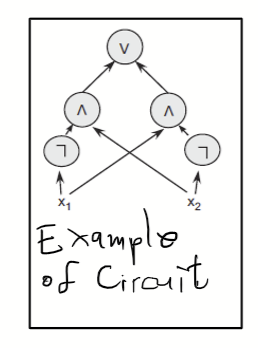
\includegraphics[width=0.2\linewidth]{images/Example-circuit.png}
    \caption{Example of a simple Boolean circuit.}
    \label{fig:enter-label}
\end{figure}

%
\begin{trailer}{Comment}
Fan-in $d>2$ 
can be simulated by a tree of $d-1 $ nodes: 
\begin{figure}[h]
    \centering
  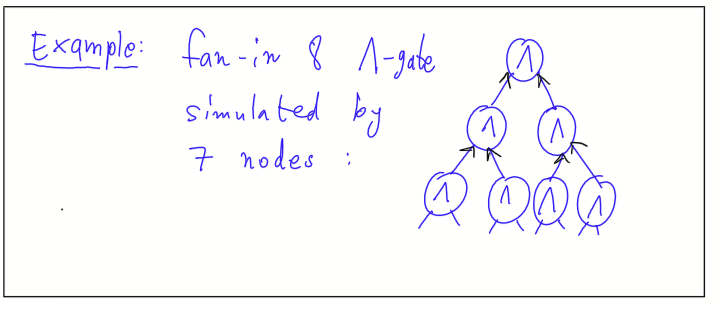
\includegraphics[width=0.5\linewidth]{images/Example-tree-circuit.png}
    \label{fig:enter-label}
\end{figure}
\end{trailer}


\newpage 

\begin{question}{What is the function computed by the circuit below?}
\begin{figure}
    \centering
    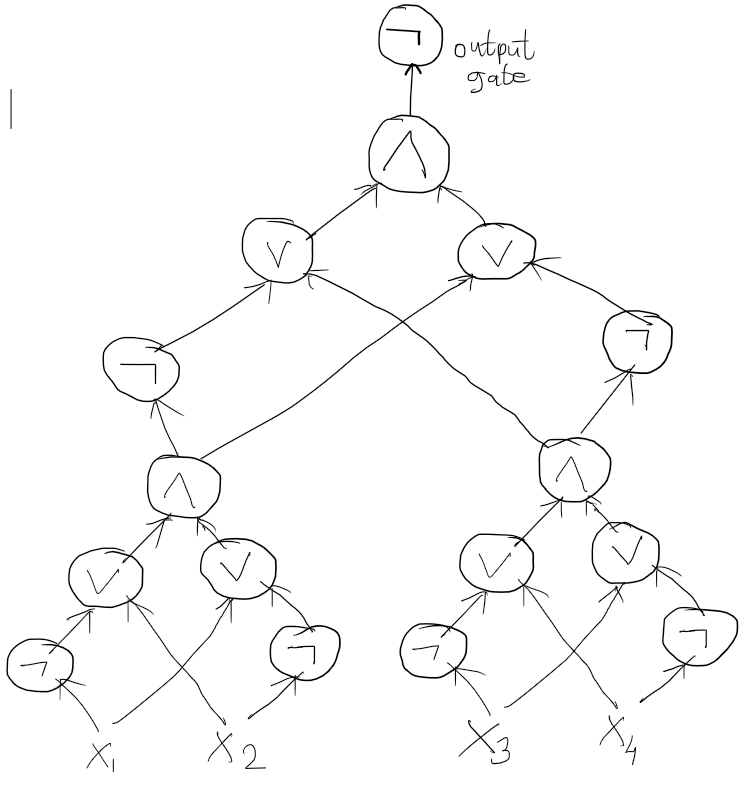
\includegraphics[width=0.75\linewidth]{images/parity-circuit-question.png}
    \caption{Question}
    \label{fig:enter-label}
\end{figure}
\end{question}

\begin{trailer}{Answer}
     PARITY on 4 input bits. It outputs 1 if the number of 1's in the input is odd. I.e., it computes the XOR of $x_1, \ldots, x_4$. In other words, it computes the function $x_1+x_2+x_3+x_4$ mod 2. (Understand why that is. Hint: recall that ${\neg x_1}\lor x_2$ is logically equivalent to $x_1\to x_2$. And notice that this structure repeats throughout the circuit.)
\end{trailer}
%\eject

\section{Circuit families, language recognition, and function computation}

Let $\mathbb{N}$ denote the set of natural numbers starting from $1$.


%\newcommand{\bits}{\ensuremath{\{0,1\}}}
%\newcommand{\demph}[1]{\textbf{\emph{#1}}}

A \emph{language} is a set of (finite) strings. Note that the language can contain infinite many strings, only that each string is finite. A \emph{string} is an ordered sequence of symbols from a fixed constant size alphabet. We shall use mainly strings over the alphabet consisting of two symbols $\bits$.
Hence, a language is simply a set $L\subseteq\bits^*$ (recall, that $\bits^*$ is the set of all finite 0-1 strings, including the empty string). 
 

\begin{svgraybox}
\begin{definition}
Let $T:\mathbb{N}\rightarrow \mathbb{N}$ be a function. 
A \emph{$T(n)$-\textbf{sized circuit family}} is a sequence $\left\{C_n\right\}_{n \in \mathbb{N}}$ of Boolean circuits, where $C_n$ has $n$ input-gates (i.e., $n$ inputs-bits) and a single output-bit such that  $\left|C_n\right| \leq T(n), \forall n \in \mathbb{N}$.\footnote{We can also define a circuit-family where some input lengths $n\in\mathbb{N}$ are \emph{skipped} in the sequence, e.g., if the length of every input should be even. We shall not use this subtlety here.}
\end{definition}
\end{svgraybox}

A language $L\subseteq\{0,1\}^*$ is said to be \emph{in} $\operatorname{\SIZE} (T(n))$, namely, $$L\in\operatorname{\SIZE} (T(n)),$$ if there is a $T(n)$-size circuit family $\left\{C_n\right\}_{n \in \mathbb{N}}$ s.t. (such that) 
$$\forall n \in \mathbb{N~} \forall x \in\{0,1\}^n: x \in L \Leftrightarrow C_n(x)=1.$$
In this case, we say that 
the family $\left\{C_n\right\}_{n \in \mathbb{N}}$ \demph{decides} the language $L$.


Similarly, for a \emph{function} $f:\{0,1\}^* \rightarrow\{0,1\}, f \in \operatorname{\SIZE}(T(n))$ if there exists $ T(n)$-size circuit family $\left\{C_n\right\}_{n \in \mathbb{N}}$ such that  $\forall n \in \mathbb{N} \quad \forall x \in\{0,1\}^n, f(x)=1 \Leftrightarrow C_n(x)=1$.
In this case, we say that 
the family $\left\{C_n\right\}_{n \in \mathbb{N}}$ \demph{computes} the function $f$.



\begin{svgraybox}
\textbf{Slice of function}. 
 Let $f:\{0,1\}^*\to\{0,1\}$ be a Boolean function.
We can consider the \emph{slice} \emph{of size} $n$ of $f$ to be the function $f_n:\{0,1\}^n\to\{0,1\}$, which is $f$ restricted to inputs of length precisely $n$. 
\end{svgraybox}

Similarly, we can consider $\left\{f_{n}\right\}_{n\in\mathbb{N}}$ to be the \textit{family} of Boolean functions $f_n:\{0,1\}^n\to \{0,1\}$, 
for all $n$ at least 1 (so, this is a family of all slices of $f$). In other words, the family $\left\{f_{n}\right\}_{n\in\mathbb{N}}$ is the sane as $f:\bits^*\to\bits$. 

\textcolor{green}{STOPPED polish Here
}






\section{Quick recap:\ growth functions, $O$-notation and run-times}

Be sure to recall the following basic definitions of (though we are not going to use them concretely in this course).

- Time bounds for Turing Machines (TMs)

- The class P (aka PTIME)

- The class NP, verifiers, short certificates

- SAT is NP complete: Cook-Levin theorem



\paragraph{Time Complexity}
We mainly consider the worst-case time for a problem to be solved by a given TM.

\begin{definition}
    Let $M$ be a $T M$ that halts on every input. Let $f: \mathbb{N} \rightarrow \mathbb{N}$ be a function, s.t., $f(n)$ is the max number  of steps it takes $M$ to halt on inputs of length $n$. We say $f$ is the running time of $M$. And that $M$ runs in time $f(n)$.
\end{definition}

\begin{trailer}{$O$-Notation}
    We usually use $n$ for the length of inputs


Recall:
\begin{enumerate}
    \item 
 $f(n)=O(g(n))$ if $\exists$ constant $c$ and $n_0 \in \mathbb{N}$ st. $\forall n \geqslant n_0 \quad f(n) \leqslant c g(n) $ (for two functions  $f, g: \mathbb{N} \rightarrow \mathbb{R}^{+}$).

\item $f(n)=o(g(n))$ if $\lim _{n \rightarrow \infty} \frac{f(n)}{g(n)}=0$
\end{enumerate}
\end{trailer}

\begin{trailer}{Basic Growth Rates}
\begin{enumerate}
    \item When $f=O\left(\log n\right)$ the base $b$ of $\log _b n$ is irrelevant.
    
    \item $2^{O(n)}$ means $\leqslant 2^{c n}$ for some $c$, const.

    \item \emph{Polynomial growth rate} means $n^{O(1)}=2^{O\left(\log n\right)}=n^c$, for some constant $c$, namely $c$ is independent of $n$ (while $n$ grows, $c$ stays fixed).
    \item \emph{Exponential growth rate} (similarly, \emph{exponential bound})  means for us $2^{n^\delta}$, for a real constant $\delta>0$. (Some texts insist that ``exponential growth'' should only refer to $2^{cn}$, for a constant $c>0$. Note the difference between this and our definition!)
\end{enumerate}
\end{trailer}






\begin{definition}[\Ppoly; polynomial-size circuits] The class \Ppoly~is the class of languages that are decidable by polynomial-size circuit families.
That is, $\Ppoly=\bigcup_{c \in \mathbb{N}} \operatorname{\SIZE}\left(n^c\right)$.
\end{definition}


\begin{theorem}
$\P \subseteq \Ppoly$.
\end{theorem}

\begin{proof}
Assignment/tutorial.
[See for a sketch in Arora-Barak'10, Sec. 6.1.1. page 110; \cite{AB09}]. 
\end{proof}

\section{Our main focus: lower bounds}

\begin{svgraybox}
\textbf{Lower bounds, hard functions}.
We say that we have a \textit{super-polynomial lower bound against \Ppoly}, namely a super-polynomial lower bound against (polynomial-size) Boolean circuits, if the following occurs: there exists a Boolean function $f:\{0,1\}^*\to \{0,1\}$ such that no polynomial-size circuit family $\left\{C_n\right\}_n$ computes $f$. In other words, $f$ is not in $\Ppoly$. If we show that $f\not\in\operatorname{\SIZE}(T(n))$, we say that we have \textit{proven a $T(n)$-lower bound for $f$} (against Boolean circuits). We say that this $f$ is \emph{hard} for $\operatorname{\SIZE}(T(n))$.
\end{svgraybox}



\paragraph{Motivation for Circuit Complexity}

1)  Non-uniformity: maybe for every $l \in \mathbb{N}$ there's a small circuit for SAT that can solve it in quadratic time?
(Karp-Lipton: PH doesn't collapse $\Rightarrow N P \subseteq P /$ poly).

2) Mathematically \textit{cleaner} than Turing Machines; so might have better hope for lower bounds.


\subsection{Most functions are hard: Shannon lower bound}

\begin{figure}
    \centering
    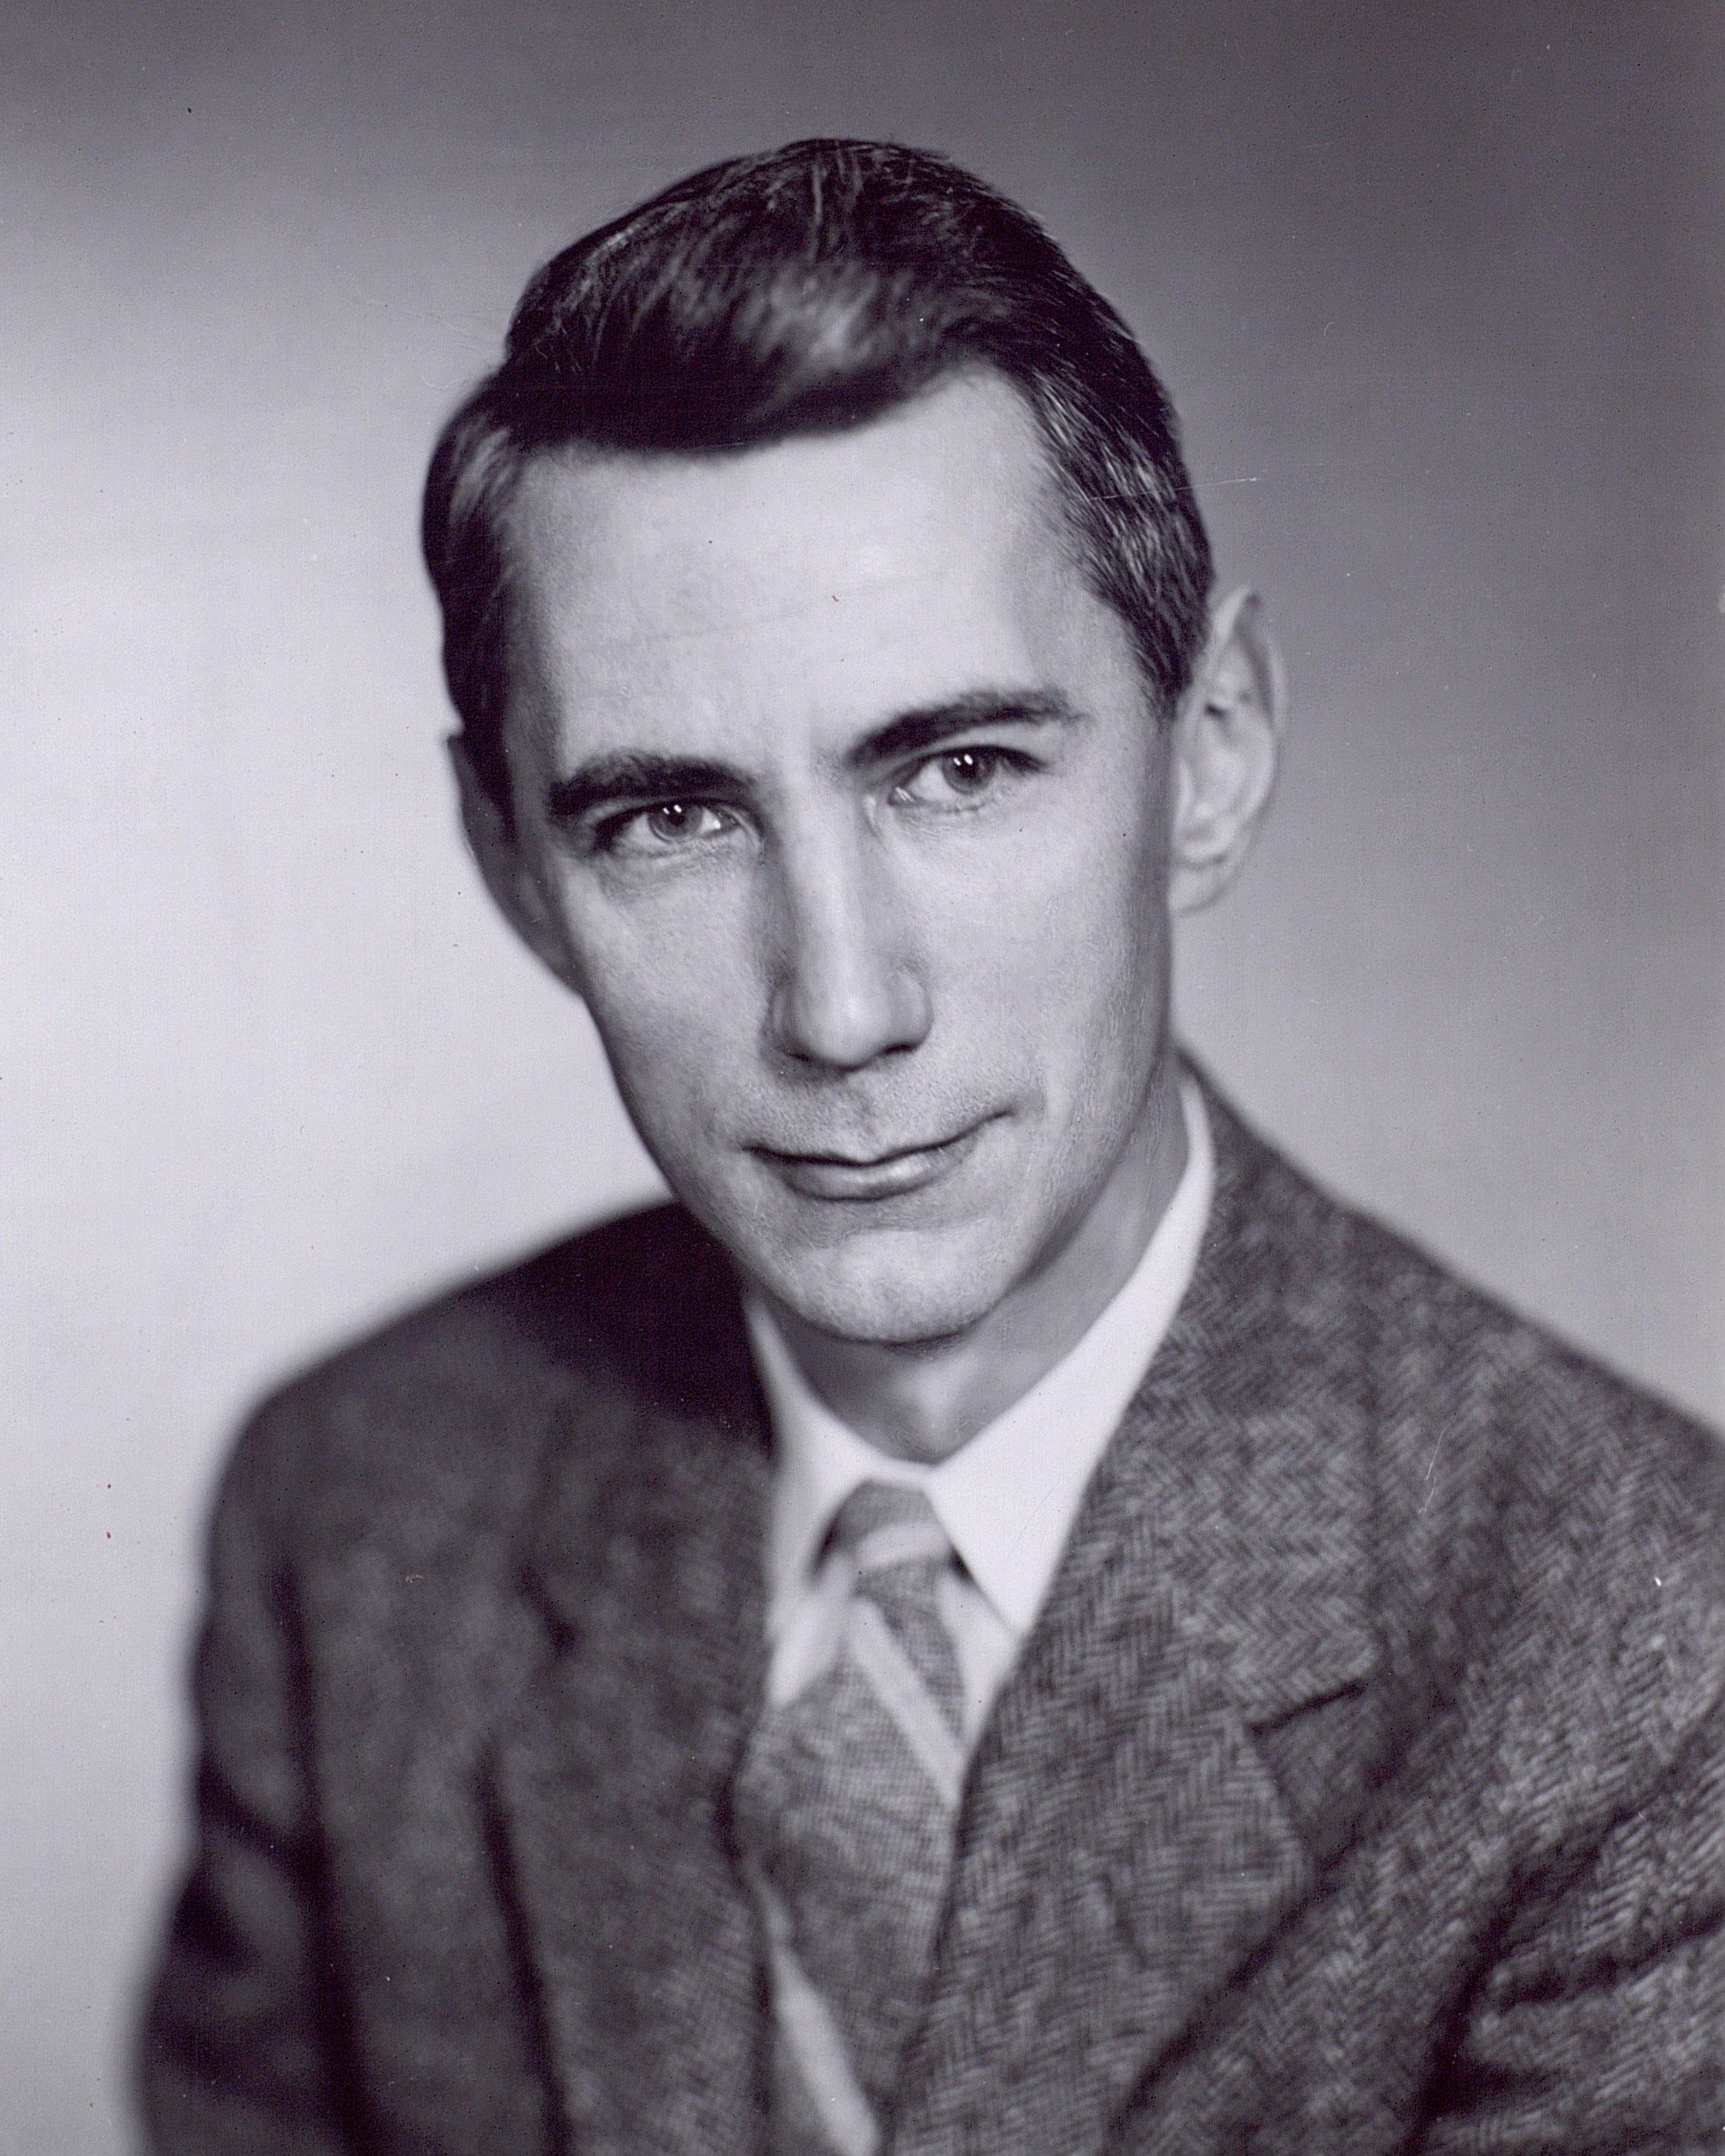
\includegraphics[width=0.25\linewidth]{images/Shannon.jpg}
    \caption{C.E.~Shannon. Source: By Unknown author - Tekniska Museet, CC BY 2.0, \url{https://commons.wikimedia.org/w/index.php?curid=144716444}}
    \label{Claude Shannon}
\end{figure}






Open: $\quad \mathrm{NEXP}\stackrel{?}{\subseteq}P/poly$ (note that by the time hierarchy theorem $\mathrm{EXP}\subsetneq P$; but in ``$\mathrm{NEXP}\stackrel{?}{\subseteq}P/poly$'' we consider NEXP which is \emph{uniform}, and P/poly which is \textit{non}-uniform).


\begin{theorem}
    [Shannon lower bound]
    For every $n>1$ exists a function $f:\{0,1\}^n \rightarrow\{0,1\}$ that cannot be computed by a circuit of size  $\le 2^n / 10 n$.
\end{theorem}

\begin{proof}[by counting method.]
\mbox{}\\

\begin{claim}
We can encode a boolean circuit of size $S$ with $9\cdot S \log S$ bits.
\end{claim}

\begin{proof}[Claim]
Using adjacency List:
\begin{figure}[H]
    \centering
    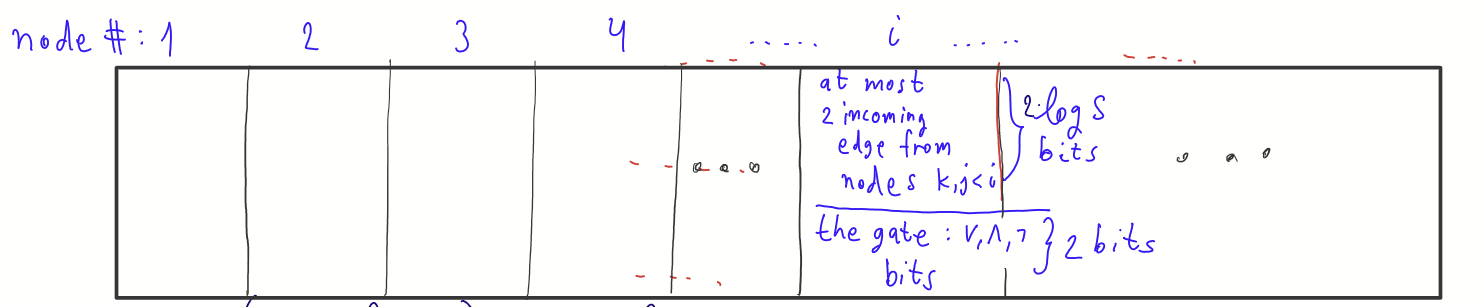
\includegraphics[width=1.1\linewidth]{images/shannon_table.png}
    \caption{Enter Caption}
    \label{fig:enter-label}
\end{figure}




We have:
$$
S \cdot(2+2 \log S) \leq 9 S \log S
.$$
(Actually, we have: 
$ 2S(\log S+1) = 2S(2 \log S) \leq 4 S \log S.
$)
\end{proof}

We now show that the number of circuits of size $\leq 2^n / 10 n$ is smaller than that of possible Boolean functions w/ $n$ inputs.
Thus, by the Pigeonhole Principle, there exists a Boolean function that cannot be computed by a circuit of size $\leq 2^n / 10 n$.

The number of circuits of size $S$ is bounded from above by the number of distinct codes of circuits of size $S$, which is
$$
\begin{aligned}
& \leq 2^{9 \cdot S \log S} \\
& =2^{\left(9 \cdot 2^{n / 10 n} \cdot \log \left(2^n / 10 n\right)\right)}=2^{\left(9 \cdot 2^n / 10 n \cdot(n-\log 10 n)\right)} \\
& \leq 2^{\frac{9 n}{10 n} \cdot 2^n}=2^{\frac{9}{10} \cdot 2^n} . 
\end{aligned}
$$
But this is 
less than $2^{2^n}$ the number of distinct Boolean functions $f:\{0,1\}^n\to\{0,1\}$. 
\end{proof}




Note: the reason we need to lower bound $2^n/10n$ circuits (and not $2^n/c$), is that encoding a circuit is super linear (i.e., $\Omega (\log n)$).




%%%%%%%%%%%%%%%%%%%%% chapter2.tex %%%%%%%%%%%%%%%%%%%%%%%%%%%%%%%%%
%
%  Monotone Circuits Lower bounds 
%
% Use this file as a template for your own input.
%
%%%%%%%%%%%%%%%%%%%%%%%% Springer-Verlag %%%%%%%%%%%%%%%%%%%%%%%%%%
%\motto{Use the template \emph{chapter.tex} to style the various elements of your chapter content.}





\chapter{Monotone Circuit Lower Bounds}
\label{sec:Razborov} % Always give a unique label
% use \chaptermark{}
% to alter or adjust the chapter heading in the running head


% Always give a unique label
% and use \ref{<label>} for cross-references
% and \cite{<label>} for bibliographic references
% use \sectionmark{}
% to alter or adjust the section heading in the running head

We've seen that proving that SAT is not in \Ppoly, i.e., can't be solved by polynomial-size circuits, implies that $\P \neq \NP$.
Due to the notorious difficulty of these questions, we are interested in proving \emph{weaker} lower bounds, namely, some lower bounds against restricted classes of circuits. 
Here, we study such a restricted circuit class: A boolean circuit without negation gates, i.e., monotone circuits.

\begin{definition}[Monotone circuit]
A Monotone circuit is a Boolean circuit that contains fan-in two gates AND and OR, but has \emph{no} NOT gates.
\end{definition}

This means in particular that monotone circuits can compute only monotone functions: a Boolean function is said to be monotone if increasing the number of ones in the input cannot flip the value of the function from 1 to 0. 

More precisely, for $\bar{x}, \bar{y} \in\{0,1\}^n$, write $\bar{x} \geqslant \bar{y}$ iff $ \forall i \in [n], x_i \geqslant y_i$, where $[n]$ denotes $\{1,\dots,n\}$. (Here, $x_i\ge y_i$ for Boolean $x_i,y_i$ means simply that $1\ge 0$ and $0\ge 0$, $1\ge 1$, while $0\not\ge 1$.)

\begin{definition}[Monotone function]
A Boolean function $f:\{0,1\}^n \rightarrow\{0,1\}$ is said to be  \emph{monotone} if $\forall \bar{x} \geq \bar{y}, f(\bar{x}) \geqslant f(y)$.
\end{definition}


Many NP problems are monotone, like CLIQUE:

Given an undirected graph $G=(V, E)$ with $n$ nodes, a $k$-clique in $G$ is a set $U\subseteq V$ of size $k$, st. every pair of nodes $u_1, u_2 \in U$ is connected by an edge (in $E$):

$$
 \forall u_1 \in u \forall u_2 \in u ( u \neq u_2\Rightarrow (u_1, u_2)\in E).
$$


Recall that a computational (decision) problem is a \emph{language}, namely an infinite set of finite strings over a finite alphabet (usually the alphabet $\{0,1\}$). Here, our language consists of all the strings that encode (in some natural way) an accepted graph, i.e., a $k$-clique with $n$ nodes.
The natural way to encode a graph in our case is this: a graph  $G=(V, E) $ with $n$ nodes, is encoded by $\binom{n}{2}$ input variables  $x_{ij}$, where the semantic of the encoding is: $x_{i j}=1$ iff $(i, j) \in E$. In other words, if the input variable $x_{ij}=1$,   our input graph contains the edge $(i,j)$, and otherwise it does not. 

We are interested in CLIQUE$(k, n)$ for a fixed $k$, as the following Boolean function: 
\begin{svgraybox}
The computational problem \textbf{CLIQUE$(k, n)$}: 

\textit{Input}: Undirected graph $G=(V,E)$ with $n$ nodes, and a number $k$ (given in unary, i.e., $1^k$).

\textit{Accept}: if the graph $G$ contains a $k$-clique. 

\textit{Reject}: otherwise.
\end{svgraybox}


 Note that $\operatorname{CLIQUE}(k, n)$ is a monotone function: If we add 1's to the input, we only \emph{increase} the chance it has a $k$-clique!
 
It is known that CLIQUE$(k,n)$ is NP-complete (see standard complexity textbooks; e.g., Papadimitriou 1994).


Since CLIQUE$(n, k)$ is a monotone (Boolean)
function we can compute it by a monotone Boolean circuit.

\begin{trailer}{Example of a monotone circuit computing CLIQUE$(n, k)$}
 ``Run" over all $\binom{n}{k} ~~ k$-sub-graphs in $G$, and check if at least one of those is a clique:

\begin{figure}
    \centering
    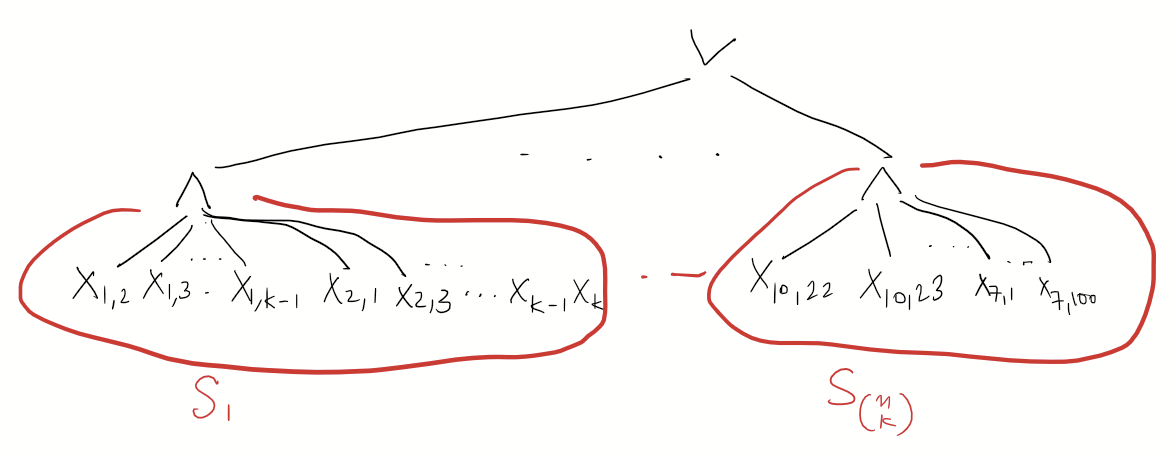
\includegraphics[width=0.75\linewidth]{images/k-clique-simple-circuit.png}
    \label{fig:enter-label}
\end{figure}

$S_1, S_2, \ldots, S_{\binom{n}{k}}$ are the $\binom{n}{k}$ subgraphs in $G$ each of size $k$.
Size of this circuit: $O\left(k^2 \cdot\binom{n}{k}\right)$.
We call such a circuit for computing $\operatorname{CLIQUE}  (n, k)$ consisting of a big $\lor$ of all $S_i$'s, each computed by $\land$'s of edges, a \textbf{\textit{crude-circuit}} for CLIQUE($n, k)$.
\end{trailer}



Notation: $CC\left(S_1, \ldots, S_{\binom{n}{k}}\right)$ is the crude circuit computing the $\lor$ of all subgraphs $S_1 \ldots S_{n\choose k }$. In general, we shall use different subgraphs: $CC\left(x_1, \ldots, x_m\right)$ for $x_i \subseteq V$ not necessarily of size $k$.


Note: When $k=w(\log n)$, $CC\left(S_1, \ldots, S_{\left(k_k\right)}\right)$ is of exponential size.
The following theorem shows this naive monotone circuit cannot be improved much:

\begin{figure}
    \centering
    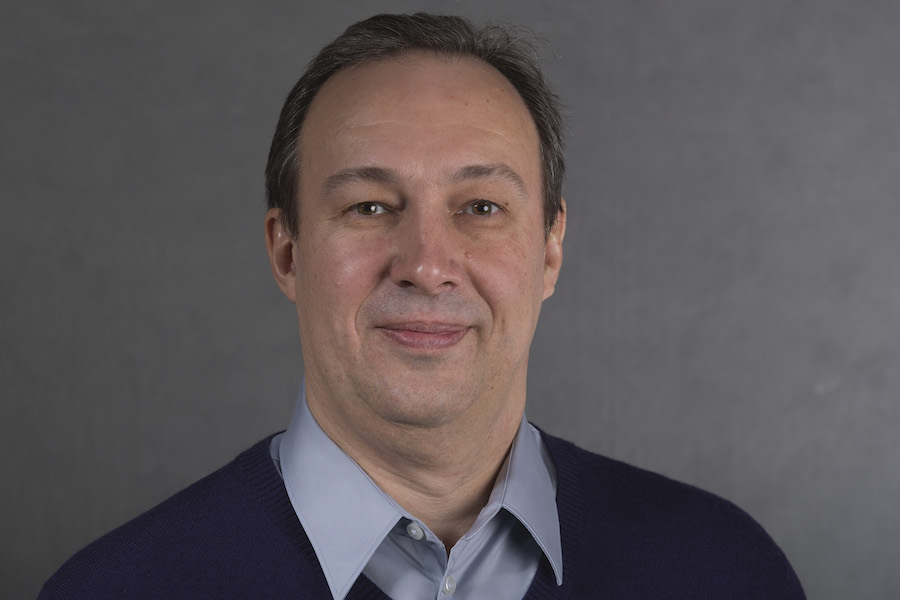
\includegraphics[width=0.25\linewidth]{images/RAZBOROV_Alexander.jpeg}
    \caption{Alexander Razborov}
    \label{fig:enter-label}
\end{figure}

\begin{svgraybox}
\begin{theorem}\label{thm:razborov}
    [Razborov] Let $k=\sqrt[4]{n}$. Then, every monotone circuit computing CLIQUE$(n, k)$ has size $2^{\Omega(\sqrt[8]{n})}$.
\end{theorem}
\end{svgraybox}
That is, exists a constant $c$ s.t. for large enough $n \in \mathbb{N}$, if $C_n$ computes CLIQUE$(n,k)$ then $\left|C_n\right| \geqslant 2^{c \cdot \sqrt[8]{n}}$.


%Recall: a crude circuit is a big OR of cliques, each computed as a big AND.



\paragraph{Approximation Method}

Here we provide an overview of the approach we take to prove \Cref{thm:razborov} which is called \emph{the approximation method}. Our exposition is taken from Papadimitriou's textbook \cite{Pap94}.
We shall describe a way of approximating any \textbf{monotone} circuit for $\operatorname{CLIQUE}({n}, {k})$ by a crude circuit, namely a big OR of cliques:

\begin{enumerate}
    
\item  Given a monotone circuit C , we shall construct a crude circuit ${CC}({X} 1, \ldots, {Xm})$ for some m and $\left|{X}_{{i}}\right| \leq l$ (for some $l$, all ${i}=1, \ldots, {m}$ ), that approximates $\operatorname{CLIQUE}({n}, {k})$ with \textbf{precision} that is dependent on the number of gates in $C$.

\item I.e., if the precision is not good, namely the crude circuit ${CC}({X} 1, \ldots, {Xm})$ for CLIQUE (n,k) we end up with makes \textit{many errors} on the CLIQUE ( $n, k$ ) function (i.e., says "NO" on an input that has a k-clique, and "YES" on an input that has no k-clique), it means that the circuit $C$ has \textit{many gates}, and vice versa.\label{it:approximation-b}

\item We show that every crude circuit ${CC}({X} 1, \ldots, {Xm})(|{X}_i| \leq l$ for some $l$, for all $i=1, \ldots, m$ ), ought to make \textit{exponentially many errors} on the function $\operatorname{CLIQUE}(n, k)$. From \ref{it:approximation-b} above we conclude that the number of gates in C was exponential.

\end{enumerate}


The \textbf{approximation} (i.e., construction of a crude circuit for CLIQUE(${n},{k})$ given the circuit $C$) will proceed in steps, one step for each gate of the monotone circuit:

\begin{enumerate}
    
\item If $C$ is a monotone circuit computing $\operatorname{CLIQUE}({n}, {k})$ we can \textit{approximate} any gate OR or AND in $C$ with a crude circuit.

\item Each such approximation step introduces rather few errors (false positives and false negatives).
\end{enumerate}


\section{Proof of monotone circuit lower bounds}

\begin{trailer}{Parameters \& notation}

Recall we want to compute CLIQUE$(n, k)$
with $n$ the number of nodes in the graph and $k$ the size of a clique within the graph. 
We set:
$$
k=\sqrt[4]{n}.
$$

\begin{svgraybox}\textbf{Goal}: Show that every monotone circuit computing $\operatorname{CLIQUE}(n,k)$ has size at least $2^{c \sqrt[8]{n}}$ for some constant $c$ (for sufficiently large $n$).
\end{svgraybox}

$$
\begin{aligned}
& l=\sqrt[8]{n} \\
& p \approx \sqrt[8]{n} \\
& M=(p-1)^l \cdot l! & \approx(\sqrt[8]{n}-1)^{\sqrt[8]{x}} \cdot(\sqrt[8]{n})! \\
& & \leq(\sqrt[4]{n})^{\sqrt[8]{n}}
\end{aligned}
$$


Each crude-circuit we use in the approximation is:

$$
C C\left(x_1, \ldots, x_m\right)
$$

for $m \leqslant M$ and $\left|X_i\right| \leqslant l, \forall i \in[m]$.

\end{trailer}

\bigskip 





- The approximation of the monotone circuit $C$ that computes $\operatorname{CLIQUE}(n, k)$ is done by induction on the size of $C$, ie., number of $\lor, \wedge$ gates in $C$.


- Comment: Such induction is also called ``Induction on the structure of $C$''.

- Such induction proceeds as follows: 


\para{Base Case} $|C|=1$, ie., $C$ consists of only a single input gate $g_{ij}$. Recall $g_{i j}$ is an input gate denoting whether $(i, j) \in E$, for $i, j \in V$.
That is, if there is an edge between $i$ and $j$ in the input graph $G$.

This is an easy case: We need to show a crude cat $\operatorname{CC}\left(X_1, \ldots, X_m\right) \mathrm{w} /$ $m \leqslant M$ and $\left|X_i\right| \leqslant l \quad \forall i \in[m]$ that
approximates $g_{i i}$ (without introducing too many errors; We shall count precisely the number of potential errors later).
But the circuit $C C(\{i, j\})=g_{i j}$ by definition. (Hence, no errors here!)


\para{Induction Step}
Given two crude circuits
$\operatorname{CC}(\mathcal X)$ and 
$\operatorname{CC}(\mathcal Y) 
$, with $\mathcal{X}=\{x_1, \ldots, x_m\}$, 
$\mathcal{Y}=\{y_1, \ldots, y_{m^{\prime}}\}$, $m\le M$, and $\left|x_i\right| \leq \ell $, for all $i$, $m'\le M $ and $\left|y_i\right| \leq \ell$, for all $i$.


We wish to construct another crude circuit  for computing $CC(\mathcal{X}) \vee CC(\mathcal{Y})$, and $\operatorname{CC}(\mathcal X) \wedge 
\operatorname{CC}(\mathcal Y)$.

\case{1}
$\lor$-gate.

Naive attempt: $\operatorname{CC}(\mathcal X)
\lor \operatorname{CC}(\mathcal Y)$ is approximated by $\operatorname{CC}(\mathcal X \cup \mathcal Y)$. That is, $\operatorname{CC}\left(x_1, \ldots, x_m, y_1, \ldots, y_m\right)$. At first glance this is a good solution because it does not introduce any errors (why?). But there is a problem: what if $m+m^{\prime}>M$?


Solution: We need to cleverly \emph{reduce} the number of sets $x_1, \ldots, x_m, y_1, \ldots, y_{m^{\prime}}$. To do this we use a combinatorial lemma called The Sunflower Lemma.

%%%%%%%%%%%%%%%%%%%%% chapter2.tex %%%%%%%%%%%%%%%%%%%%%%%%%%%%%%%%%
%
%  
%
% Use this file as a template for your own input.
%
%%%%%%%%%%%%%%%%%%%%%%%% Springer-Verlag %%%%%%%%%%%%%%%%%%%%%%%%%%
%\motto{Use the template \emph{chapter.tex} to style the various elements of your chapter content.}










\chapter{Constant Depth Circuit Lower Bounds}
\label{hastad} % Always give a unique label
% use \chaptermark{}
% to alter or adjust the chapter heading in the running head

%\section{Defining constant depth circuits}

Recall \Cref{def:boolean-circuit} of Boolean circuits.
We define the \emph{\textbf{depth}} of a Boolean circuit $C$ as 
the maximal length (i.e., number of edges) in a path from 
a leaf to the output node.

Here is an example of a circuit of depth 3:
\begin{figure}
    \centering
    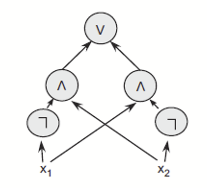
\includegraphics[width=0.2\linewidth]{images/depth_3_circuit.png}
    \label{xxx}
\end{figure}

\newcommand{\complexityclass}[1]{\sf{#1}}
\newcommand{\ACZ}{\ensuremath{\complexityclass{AC}^0}}


Recall that we are interested in the  study of the asymptotic size of circuit families, not a single circuit. That is, we want to consider how circuit size grows when the number of inputs $n$ grows. In this chapter we shall focus on circuit families $\{C_n\}_{n=1}^\infty$
whose number of inputs bits $n$ grows, their size $|C_n|$ grows polynomially while their depth is \emph{fixed} throughout the family, namly is a constant $c$ independent of $n$. 

%The class of Boolean functions computed by such circuit families is denoted $\ACZ$, and the class of such constant depth cir

%We can consider circuits of constant depth. This means that the depth of the circuit is \emph{independent of the number of inputs} $n$. In other words,  while $n$ the number of input gates can grow to infinity in the Boolean circuit family $\{C_n\}_{n=1}^\infty$, the depth of each circuit $C_n$ stays the same!


If the depth of the circuit is constant and the fan-in of gates is at most two, then the number of functions we can compute with such constant-depth circuits is constant. For example, the number of variables (appearing as leaves, i.e., input nodes) is constant that way, so for a large enough number of inputs $n$, we will not be able to compute functions that read all the $n$ inputs. This means that the model is \emph{not  complete}: for a constant $d$, a depth-$d$ circuit cannot compute all Boolean functions over $n$ inputs for every $n \in \mathbb{N}$.

To solve this problem and make the model of constant-depth
circuits meaningful we allow \textbf{\textit{unbounded} \emph{fan-in}} gates: unbounded fan-in AND gates: $\left(\varphi_1 \wedge \varphi_2 \wedge \ldots \wedge \varphi_\ell\right)$, and unbounded fan-in OR gates
$\left(\varphi_1\lor \cdots \lor \varphi_{\ell}\right)$, where the $\varphi_i$'s are circuits (of constant depth) by themselves, with possibly \emph{joint} nodes. 
\begin{figure}
    \centering
    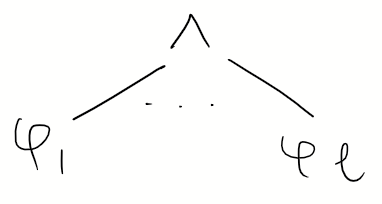
\includegraphics[width=0.2\linewidth]{images/AND.png}
    
\includegraphics[width=0.25\linewidth]{images/OR.png}
    \caption{Illustration of unbounded fan-in AND and OR gates.}
\end{figure}



\newcommand{\depth}{\ensuremath{{\rm depth}}}

\begin{definition}[Depth-$d$ circuit family, constant-depth family]
\label{def:constant-depth-circuit}
A circuit family 
$\left\{\mathrm{C}_n\right\}_{n=1}^\infty$ with unbounded fan-in $\land,\lor$ gates and fan-in one negation gate is said to be of \emph{depth-$d$}, if the depth of $C_{n}$ is $d$, for all $n\in\N$. We denote by $\depth(C_n)$ the depth of the circuit $C_n$.
If $d$ is a constant (independent of $n$) we call $\left\{C_n\right\}_{n=1}^\infty$ a \emph{constant-depth family of circuits}.
\end{definition}

\textbf{Notation}: \ACZ\ denotes the complexity class 
consisting of all the functions $f:\{0,1\}^* \rightarrow\{0,1\}$ computable by  constant-depth circuit families  (equivalently, all decision problem decidable by \ACZ\ circuit families).

\para{Alternating Formulas}


We are going to use the following ``normal-form'' for constant-depth circuits. This is done for the sake of simplicity, and does not change the size of the circuits significantly, as we remark below.


A Boolean circuit is said to be an \emph{alternating  formula} if it is a formula (i.e., the underlying circuit graph is a tree), and every OR gate is followed by an AND gate followed by an OR gate, etc. Moreover, all negations in an alternating formula are pushed to the bottom of the circuit: that is, a negation node can only be connected to an input node (and that input node is not connected to any other node except a negation node). 
Here is an illustration:
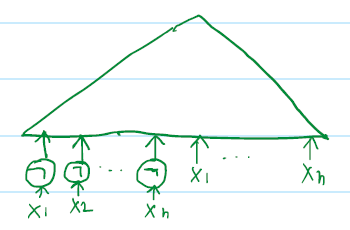
\includegraphics[width=0.3\textwidth]{image004.png}


% Always give a unique label
% and use \ref{<label>} for cross-references
% and \cite{<label>} for bibliographic references
% use \sectionmark{}
% to alter or adjust the section heading in the running head

For simplicity, we can assume that a constant-depth circuit has two types of inputs: every variables $x_i$ has a negative copy $\overline x_i$ (thus, getting rid of the need to specify a negation gate explicitly).  

Note that in an alternating formula every \emph{layer} (equivalently, \emph{level}) of the circuit, namely, nodes of a given depth $l$, are all of the same type: either all $\land$, all $\lor$ or all input variables (positive or negative).



We shall assume that all \ACZ\ circuits are alternating formulas:


\begin{tcolorbox}[colframe=white, colback=gray!11, boxrule=0mm, sharp corners]
 \textbf{Important:} From now on, when speaking about constant-depth circuits (i.e., \ACZ\ circuits), we assume by default the fan-in of $\lor, \land$ gates  is \emph{unbounded} ($\neg$ has fan-in one), and the circuits are \emph{alternating formulas}, and the \textbf{depth} is defined as maximal number of alternations between $\land$ and $\lor$ gates (or vice versa), namely the number of layers in the formula,  excluding the bottom layer which contains only the input variables (positive or negative).  
\end{tcolorbox}

\begin{exercise}
Show that every depth-$d$ circuit can be transformed into an alternating formula of depth-$O(d)$ circuit and with all negation gates on the leaves, with a polynomial size increase only.

\noindent---

\noindent{\small Hint: we can "unwind" the circuit into a formula (a tree; that is, if we used a subcircuit more than once [namely, it has out-degree more than 1], we copy this subcircuit for each such usage). Because the depth is constant this will increase the size of the circuit by at most a polynomial (exponential in a constant---i.e., polynomial). To make the formula alternating, first push all the negation to the bottom, using \emph{de Morgan rules}. And then, add dummy edges and gates to make every path from leaf to the output gate alternating between OR and AND. These all incur a polynomial increase in size.
}
\end{exercise}



\newcommand{\Parity}{\ensuremath{\operatorname{PARITY}}}

%\section{Lower Bounds Against Constant-Depth Circuits for PARITY}

\section{The PARITY Function}

The function PARITY determines the parity of the total number of ones in the input bits:

\begin{tcolorbox}[colframe=white, colback=gray!11, boxrule=0mm, sharp corners]
$
\Parity(x_1,\dots,x_n): =
\begin{cases} 
1 & \text{if the number of 1's in } (x_1, x_2, \dots, x_n) \text{ is odd}, \\
0 & \text{if the number of 1's in } (x_1, x_2, \dots, x_n) \text{ is even}.
\end{cases}
$
\end{tcolorbox}

Equivalently, $\Parity$ is defined as the XOR of the input bits, denoted $x_1\parity\cdots\parity x_n$. Another equivalent definition is using modulus: $x_1+\cdots+x_n = 1 \mod 2$.

We denote by $\Parity_n$ the \Parity\ function restricted to inputs of length precisely $n$.

The main result in this chapter is the following:


\begin{tcolorbox}[colframe=white, colback=blue!11, boxrule=0mm, sharp corners]
\begin{theorem}[\ACZ\ lower bound for \Parity]
\label{thm:ACZ-lower bound}
Every circuit family of depth-$d$ computing the $\Parity_n$ function requires size $2^{\Omega\left(n^{\nicefrac{1}{(d-1)}}\right)}$.
\end{theorem}
\end{tcolorbox}



Note: this means that if $d$ is constant, then the size lower bound is exponential: $2^{\Omega\left(n^{\nicefrac{1}{(d-1)}}\right)}=
2^{\Omega\left(n^k\right)}$, for some constant $0<k<1$.

The theorem is a consequence of the fact that every function in \ACZ\ can be reduced to a constant function by setting relatively few variables to constants.
The proof uses the Random Restriction Method described in the sequel.

\section{The Skeleton of the Lower Bound Argument}



\begin{tcolorbox}[colframe=white, colback=gray!5, boxrule=0mm, sharp corners]
\textbf{Upshot of argument}: The idea is to randomly restrict (assign) the variables of the circuit (of which we want to show it cannot compute \Parity). If the circuit is small, such a restriction collapses (gradually) the depth of the circuit to a depth-2 circuit. If the depth of the initial circuit was constant, this gradual step-by-step depth reduction needs to be done only for a constant many times. If we made random assignments (restrictions) only for a constant many times, we can rest assure that we have not assigned (i.e., fixed) too many variables. Hence, the function $\Parity$ under these restrictions still has a lot of free variables. But such $\Parity$ with sufficiently many free variables cannot have small depth 2 circuits (this we show by an auxiliary elementary argument).
\end{tcolorbox}

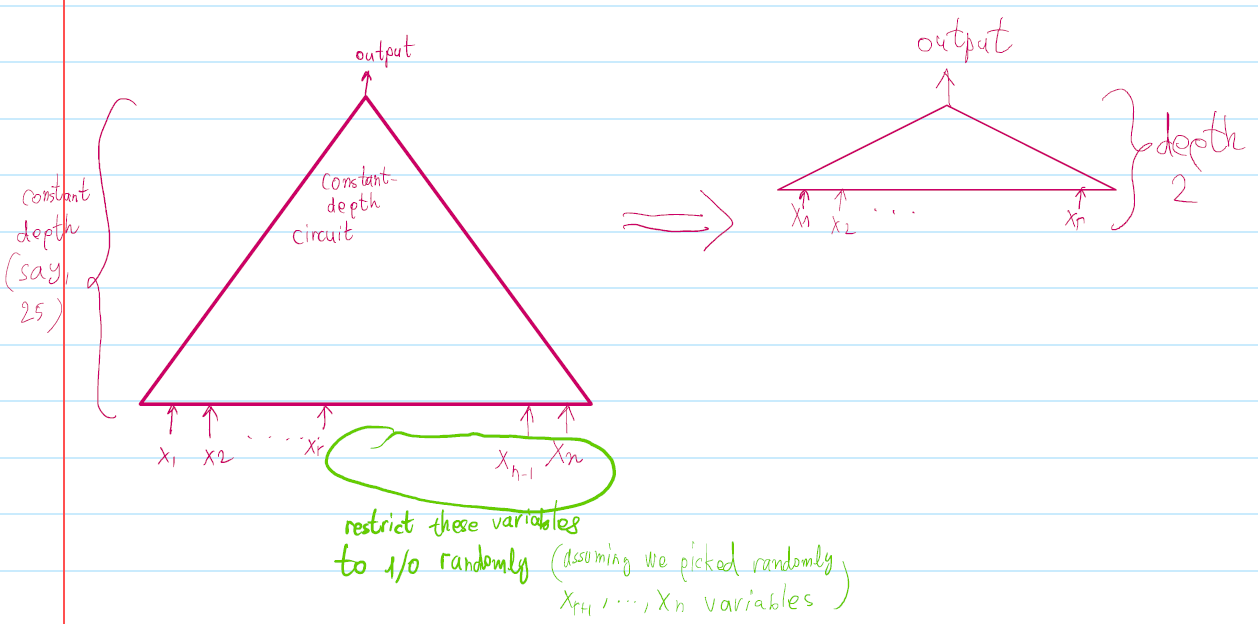
\includegraphics[width=0.9\textwidth]{images/image007.png}


\begin{note} Notice the similarity with the monotone circuit lower bound proof: we use structural induction on the circuit purported to correctly compute \Parity. \end{note}

\medskip
Here are the main steps of the argument with slightly more detail.

\para{Random Restriction Method: Structure of Argument}

\begin{enumerate}
\item By  way of contradiction, start with a purported small depth-$d$ circuit $C$ for $\Parity_n$.
We are going to assign to some of the input variables of the circuit $C$ (and hence, also to the function $\Parity_n$ it is supposed to compute), random 0,1 values. We show the result of these assignments leads to conflicting effects: with high probability, while the circuit restricted to these randomly chosen partial assignments becomes a circuit that computes a very simple function, the function $\Parity$ is still a rather complicated function to compute even after all these restriction.
\item Let $\overline x$ be $n$ variables $x_1,\dots,x_n$. Pick a random assignment $\rho_0: \overline x \rightarrow\{0,1, *\}^n$ with ``$x_i \rightarrow *$'' meaning that $x_i$ is \emph{un-assigned}, namely, stays a \emph{free} variable. We make sure that enough $x_i$'s stay  free, as this is crucial to get our contradiction.
\label{it:two-165}

\item Depth Reduction Step: 
%\item   $f$ is resilient in the sense that $f\rst\rho
%%\not\equiv 0$;

\begin{enumerate}
\item 
If $C$ is a small circuit then the \emph{function} computed by $C\rst\rho_0$, namely the restriction of $C$ to the assignment $\rho_0$, has a depth  $d-1$ circuit of small size. 

\item
Sequentially we assign new further random restrictions $\rho_1,\dots,\rho_{d-3}$
 (extending $\rho_0$) so that we reduce the depth of $C$ by 1 each time, until the depth is 2.
\end{enumerate}

\item 
At this point, we end up with a circuit $C^{\prime}$ of depth 2, namely a $k$-DNF or a $k$-CNF, for some small $k$ that computes the function 
$\Parity_n\rst\rho_0\rho_2\ldots\rho_{d-3}$.

\item
We now use an auxiliary statement to reach a contradiction: since we made sure that each assignment $\rho_i$ leaves enough variables free, 
$\Parity_n\rst_{\rho_0\rho_2\ldots\rho_{d-3}}$ is the PARITY function on $k'$ variables, i.e., $\Parity_{k'}$. But this is still a relatively "complex" function:
in particular, it is a very simple argument to show that there are no $k$-CNF formulas for $\Parity_{k'}$, whenever $k'>k$, which will conclude the argument.
\label{it:final-step:269}
\end{enumerate}


\begin{figure}
    \centering
    \includegraphics[width=0.4\textwidth]{images/hastad-sitter-600.jpg}
    \caption{Johan H\aa stad}
\end{figure}


\subsection{Depth Reduction Step: the Switching Lemma}

We shall use the following notation.
\begin{itemize}
    \item \textit{Boolean (propositional) variables:} \(x_1, x_2, \ldots \).
    \item \textit{Literal:} \(x_i\) or \(\neg x_i\) (i.e., a variables or its negation).\\
    A negation of a variable  \(x_i\) is written as eiter \(\neg x_i\), or $\overline {x_i}$.
    \item \textit{Clause:} A disjunction of literals.\\
    Example: \((x_1 \lor \neg x_2 \lor x_3)\)
    \item \textit{CNF:} Conjunctive Normal Form formula, namely a conjunction  of clauses.\\
    Example: \((x_1 \lor \neg x_2 \lor x_3) \land (x_1 \lor x_4 \lor x_5) \land (x_2 \lor \neg x_7 \lor \neg x_{20} \lor \neg x_{102})\)
    \item \textit{DNF:} Disjunction Normal Form formulas, namely a disjuncion of ANDs of literals (an AND of literals is sometimes called \emph{a term}.\\
    Example: \((x_1 \land x_4 \land x_7) \lor (x_8 \land \neg x_9 \land x_{10}) \lor (x_3 \lor \neg x_2)\)
    \item \textit{$t$-clause:} A clause with at most \(t\) literals.\\
    Example: 3-clause: \((x_1 \lor \neg x_2 \lor x_7)\)
    \item \textit{$t$-CNF:} A CNF with all clauses being \(t\)-clauses.
    \item \textit{$s$-DNF:} A DNF with all terms  having at most \(s\) literals.
\end{itemize}


The below figure illustrates a single Depth Reduction Step. Such a step is also called  ``Switching'', as it switches a $t$-CNF into an $s$-CNF, or vice versa.

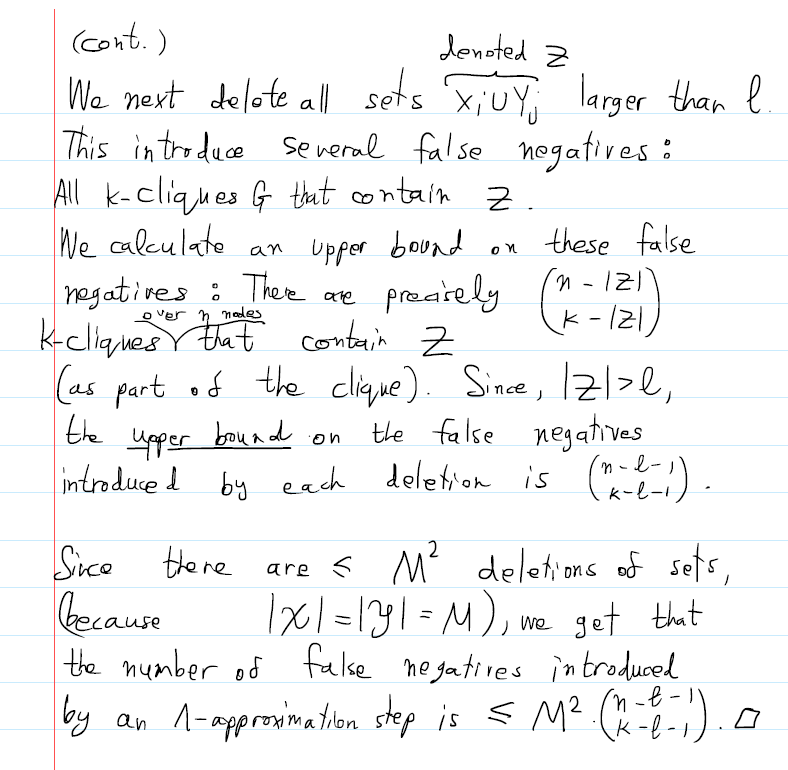
\includegraphics[width=0.7\textwidth]{images/image008.png}

\begin{note} We can always turn a $t$-CNF into an $s$-DNF for some \textit{big} $s$ (by distributing out \(\lor, \land\) using de Morgan's rules).
But then we've not maintained the invariant that the bottom level has fan-in \(\leq s\) (namely, \(s\) is small enough).
In other words, we will end up with a depth-2 circuit, but of huge size computing \(f\rst_\rho\). This will not give us a contradiction since every function is computable by an exponential-size circuit.
\end{note}

\para{Examples of Assignments and their Consequences}
\emph{How can we  turn a $t$-CNF into an $s$-DNF while keeping $s$ small}?
We can turn the $t$-CNF to a (general) DNF using de Morgan rules (just distribute $\wedge$ over $\vee$), for example
\[
(x_1 \vee \bar{x}_2) \wedge (x_3 \vee \bar{x}_4) \equiv (x_1 \wedge x_3) \vee (x_1 \wedge \bar{x}_4) \vee (\bar{x}_2 \wedge x_3) \vee (\bar{x}_2 \wedge \bar{x}_4),
\]

and then try to \emph{eliminate literals} in big ANDs by using assignments to the literals in those terms. This may reduce indeed the size of terms, and if we do this enough we may be able to reduce all the terms that are wider than $s$.
 
 
Consider the following DNF:
\[
(x_1 \wedge x_2 \wedge \bar{x}_3 \wedge \bar{x}_5 \wedge \bar{x}_8) \vee ( \dots \wedge \bar{x}_9 \wedge \dots)\lor\dots.
\] We can assign $1$ to $x_2$ and $1$ to $x_9$. In the first conjunct (i.e., the first AND or term) it results in the \emph{deletion of $x_2$}, while in the second conjunct, it results in \emph{deletion of the whole conjunct}:

Assigning $1$ to $x_2$:
\[
(x_1 \wedge x_3 \wedge \bar{x}_5 \wedge \bar{x}_8) \vee ( \dots \wedge \bar{x}_9 \wedge \dots )
\]
Assigning $1$ to $x_9$:
\[
(x_1 \wedge x_3 \wedge \bar{x}_5 \wedge \bar{x}_8) \vee \underbrace{( \dots\wedge 0 \wedge \dots)}_{\text{false}} 
\]





\begin{note}\
\begin{enumerate}
    \item Literal $l_j \from 0$ (i.e., assigning $0$ to literal $l_j$)
    \[
        (l_j \wedge D) \equiv \text{false}.
    \]
    So the whole AND disappears.
    
    \item Literal $l_j \from 1$:
    \[
        (l_j \wedge D) \equiv D.
    \]
    So we reduced the size of the AND by $1$.
\end{enumerate}
\end{note}

But how can we choose the assignment of $0$ and $1$'s to variables that guarantees eliminating all the large conjuncts, without fixing all the variables in the DNF formula (recall that by \Cref{it:two-165} above we need to keep sufficiently many variables $x_i$ free)?
The idea is to use the \emph{probabilistic method}: choosing a \emph{random} $g: \overline x \to \{0,1, *\}^n$ will lead with \textbf{positive} probability to an assignment that eliminates \emph{all} large conjuncts, while leaving enough variables free. When an event occurs with a positive probability, in this case the event of choosing an assignments with the desired properties, it means that there \textbf{exists} at least one such assignment. This will be enough for our purpose: the existence of such an assignment is sufficient to conclude our proof, because our argument hinges on a proof by contradiction: if there exists a small constant-depth circuit for PARITY, then there \emph{exists} also a desired assignment (formally, a sequence of assignments) that will yield our contradiction as in \Cref{it:final-step:269}.

\para{Switching via Random Restrictions}

\textbf{Notation:} 
\begin{enumerate}
\item 
 A \textit{restriction} $\rho$ for $l$ variables in $\bar{x}$ is a function $\rho: \bar{x} \to \{0,1, *\}$, assigning either 0, 1 values to the variables or leaving them free, namely $\rho(x_i) = *$ means that $x_i$ is \textit{unassigned} (or ``free'') according to $\rho$.

 
\item For a function $f: \{0,1\}^n \to \{0,1\}$ and a   restriction $\rho: \bar{x} \to \{0,1, *\}$, we write $f\upharpoonright \rho$ to denote the function $f$ where the variables are set according to $\rho$.
%and $\rho(x_i)$ means $x_i$ is \textit{left unassigned}.

If we then apply another restriction $\tau$ to the variables in $f\upharpoonright \rho$, we 
write $f\upharpoonright_{\rho\tau}$ to denote $(f\upharpoonright \rho)\upharpoonright \tau$. In other words,
\[
f\upharpoonright_{\rho\tau} = f\upharpoonright_{\rho \cup \tau}
\]
where $\rho \cup \tau$ is the union of two functions.
\end{enumerate}



\begin{tcolorbox}[colframe=white, colback=green!6, boxrule=0mm, sharp corners]
\begin{definition}[Random Restriction]\label{def:random-rest}
 Let $0< p<1$.
Let $\cR$ be a distribution on partial restrictions $\rho$ to the variables $\overline{x}$ with $|\overline{x}|=n$ , as follows.
$$
\begin{aligned}
& ~~~~~~~~~~~ \quad \operatorname{Pr}\left[\rho\left(x_i\right)=*\right]=p \\
& \operatorname{Pr}\left[\rho\left(x_i\right)=0\right]=\operatorname{Pr}\left[\rho\left(x_i\right)=1\right]=\frac{1-p}{2}.
\end{aligned}
$$
\end{definition}
\end{tcolorbox}
In other words, we pick randomly and independently for each variable $x_i$ with $i\in[n]$, either to leave it free with probability $p$, or to fix it to 1 or 0 with equal probability $(1-p)/2$.


\begin{tcolorbox}[colframe=white, colback=blue!5, boxrule=0mm, sharp corners]
\begin{theorem}[Switching Lemma]\label{thm:Switching-Lemma}
For every positive integers $r$ and $k$ and $n$, if a Boolean function $f$ with $n$ variables is computable by an $r$-DNF and $\rho$ is a random restriction as above with $0<p \leq \frac{1}{9}$, then with probability at most $(9pr)^s$, $f\!\rst_\rho$ \emph{cannot} be computable by  an $s$-CNF.
\end{theorem}
\end{tcolorbox}

The Switching Lemma thus shows that the ``bad'' event of a function computed by an $r$-DNF formula not being able to switch, under  a random restriction,  to a function that can be computed by an $s$-CNF, is small. This would mean that with high enough probability the ``good'' event happens: a random assignment switches an $r$-DNF to an $s$-CNF.
In practice, we usually need to have the probability of the bad event to be \emph{really} small, in this case  exponentially small, so that the probability that \emph{none} of a collection of bad events happens in the random experiment is small (using the union bound), and specifically smaller than 1, to be able to claim there exists an object with the required properties (in our case, an assignment that would switch exponentially many $r$-DNFs).  

However, we note that this probabilistic argument via the union bound  is  \emph{not} sufficient to conclude the argument. We shall also need to make sure that such a ``good'' random assignment  \emph{leaves many variables free}. For this purpose, we will use a common tool in probabilistic analysis and concrete complexity: \emph{concentration bounds} (in our case it will be the Chernoff Bound). We  explain this point in the the next section when proving the lower bound.


\begin{exercise} Show that by applying the Switching Lemma to the function $\neg f$ we can get the same result with the terms ``DNF'' and ``CNF'' interchanged. Namely, the probability that an $r$-CNF does not switches to an $s$-DNF is at most $(9pr)^s$.
\end{exercise}

\section{Proof that PARITY does not have small circuits, using the Switching Lemma}

Recall that we want to prove \Cref{thm:ACZ-lower bound}  stating that every circuit family of depth-$d$ computing the PARITY on $n$ variables requires size $2^{\Omega\left(n^{\nicefrac{1}{d-1}}\right)}$.

So, suppose  that $C$ is a depth-$d$ alternating formula circuit of size $S$ computing $\Parity_n$. We can assume that 
$S< 2^{ n^{\nicefrac{1}{d-1}}}$, as otherwise we finish the proof.


Recall that we assume that $C$ is an alternating formula, with $d$ layers, where in each layer all gates are either $\land$ or $\lor$.  The proof proceeds by first a ``preprocessing step'' in which we use the Switching Lemma to decrease the fan-in of the \emph{bottom} layer gates, followed by   $d-2$ depth reduction steps using the Switching Lemma in which we gradually reduce the depth of the circuit, from bottom to top, by one depth, until we reach a depth-$2$ circuit.
After this, we can conclude the theorem: if the circuit was too small, we end up with a $k$-CNF (or $k$-DNF) computing \Parity\ over more than $k$ variables which is easily shown to be impossible.




% Enable watermark from this point onward
%\SetWatermarkText{DRAFT}



\para{Decreasing Bottom Layer Fan-in}

This step is needed in order to optimise the lower bound, namely to reach the tight lower bound of $2^{\Omega(n^{1/d-1})}$ (see \Cref{note:bottom-explanation}).

Consider the bottom two layers of the given constant-depth circuit. We assumed that the layers alternate between $\land$ and $\lor$, thus the depth-2 sub-formulas  at these bottom two layers are all either DNFs or CNFs. Let us assume  without loss of generality  that they are all CNFs. The bottom fan-in of these CNFs may be large, namely, it may be $\ell$-CNFs for a large $\ell$. 
Since  $\ell$ may be  very large, using the Switching Lemma to turn this $\ell$-CNF to an $s$-DNF will be too expensive, in the sense that applying the Switching Lemma with this $\ell$ would give us probability of $\leq (9p\ell)^s$, but with \emph{large} $\ell$, which later would mean we get a weaker lower bound (e.g., we would get a lower bound of $2^{\Omega(n^{\frac{1}{d}})}$, which is weaker, namely smaller, than our lower bound of $2^{\Omega(n^{\frac{1}{d-1}})}$).
See \Cref{note:bottom-explanation} for an explanation of this. 



For this reason, we shall reduce the fan-in of the bottom layer (i.e., layer 1) directly using the Switching Lemma (while maintaining a lower probability of failure).

\begin{claim}\label{cla:bottom-switch}
An $\ell$-CNF does not turn into a $k$-CNF under a random restriction $\rho$ with probability $\leq (9p_0)^k$, for $p_0$ the probability a variable is free in the random restriction $\rho$. Specifically, when $k = 2 \cdot \log S$, if we choose $p_0 = \frac{1}{18}$, the probability of failure is at most $ \frac{1}{S^2}$.
\end{claim}

\begin{proof}[Claim]
The below figure illustrates  the simple argument:

\begin{center}
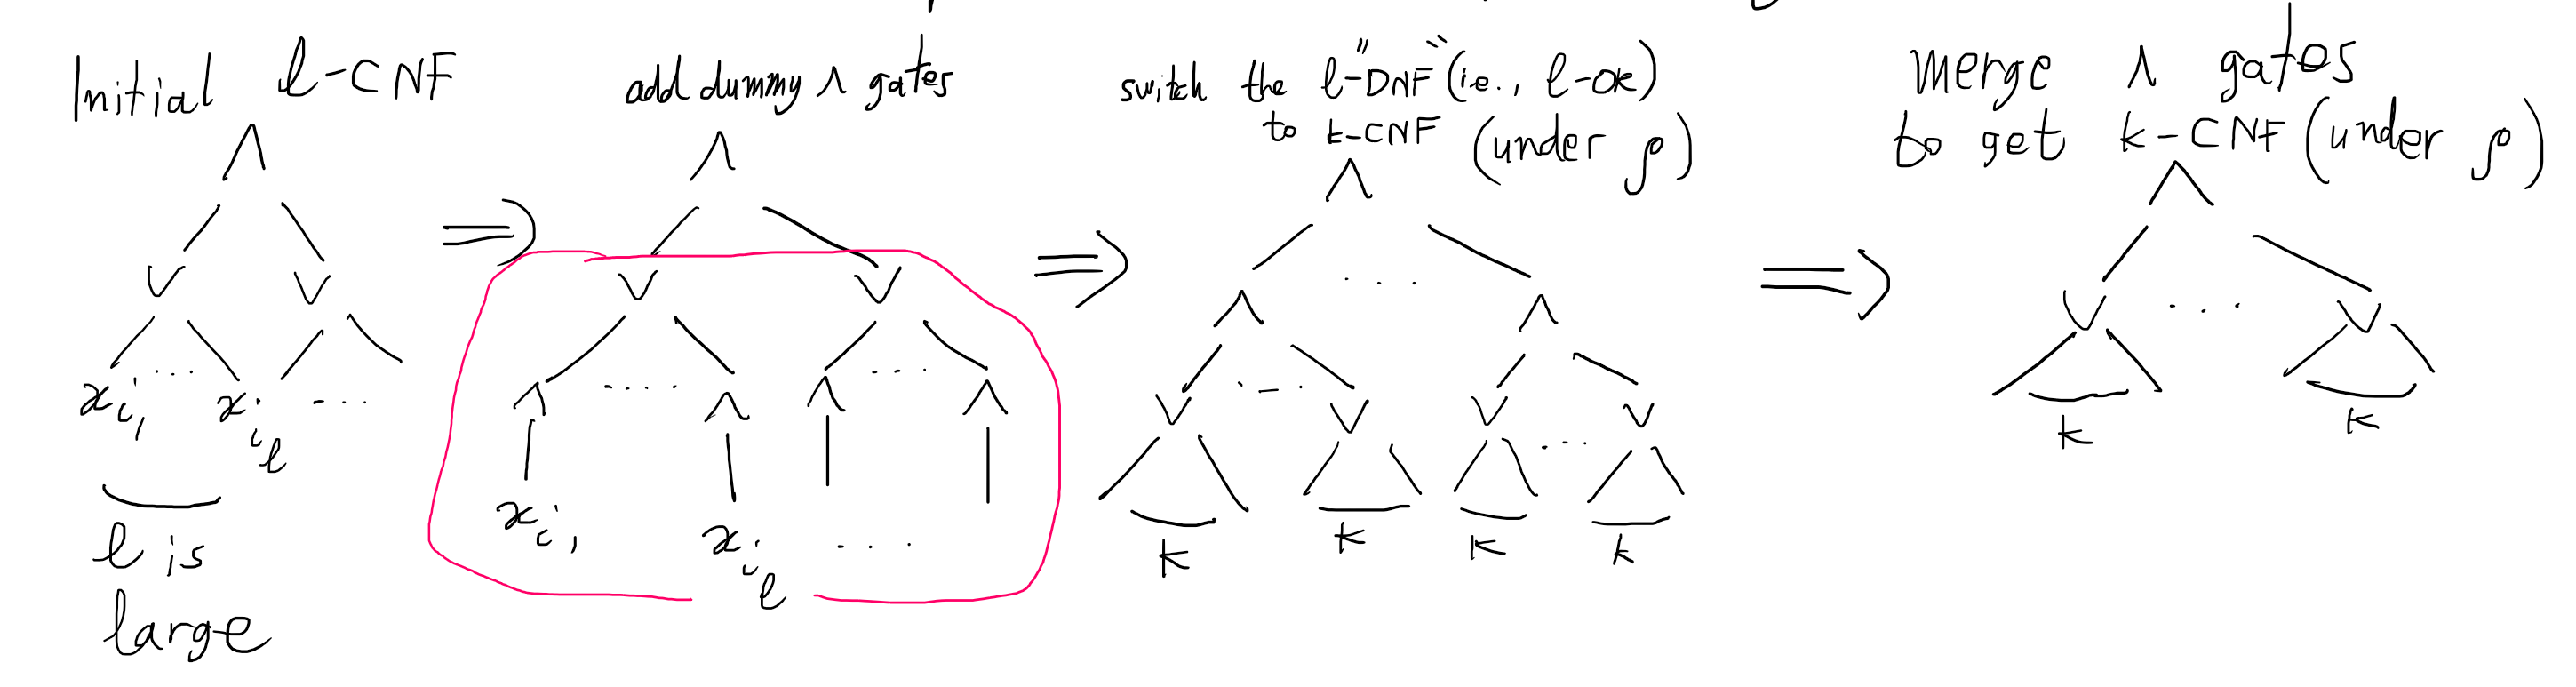
\includegraphics[width=\textwidth]{images/bottom-layer-switch.png}
\end{center}


In particular, we switch the lower 1-DNFs (\emph{in red}) into $k$-CNF with a random restriction, so by the Switching Lemma, the probability the switching fails is 
\[
\leq (9 \cd p_0 \cd1)^k = (9 \cdot \frac{1}{18})^{2 \cdot \log S} = \frac{1}{2^{2 \cd\log S}} = \frac{1}{S^2}.
\]
\
\end{proof}

By this claim, and using the union bound, the probability that at least one $\ell$-CNF in layer 2 does not switch is at most $ S\cd 1/S^2 = 1/S$.



\para{Repeated Depth Reduction Steps}
We now start from a circuit $C{\rst}_{\rho_1}$ with $k$-CNF at the bottom, for $k = 2 \log S$.
We go by induction on depth, to prove the following.


\begin{tcolorbox}[colframe=white, colback=red!11, boxrule=0mm, sharp corners]
\begin{lemma}[Induction Statement]\label{lem:induction-switch}
Let $C$ be a depth at least $d$ circuit of size 
$S<
2^{
\sqrt[d-1]{n}
}$ 
with layer-1 (bottom) gates all of fan-in  $ \leq k=2 \log S$ (either  $\land$ or $\lor$),
with $n$ input variables  
$\overline x$ (with positive and negative copies). Assume that the gates in layer $d$ are all $\land$ gates (resp., $\lor$ gates). 
Then, there exists a restriction $\rho: \overline {x} \rightarrow\{0,1, *\} $ with at least  $\frac{p^{d-2} \cdot n}{2^{d-2}} $ free variables, where $ p=\frac{1}{36 \cdot \log S}$, such that  
the function computed by $g{\rst}_{\rho}$ for every $\land$ (resp. $\lor$) gate in layer $d$ is computable by a $k$-DNF (resp., a $k$-CNF) formula. 
\end{lemma} 
\end{tcolorbox}

\begin{proof}[\Cref{lem:induction-switch}]
We prove it for the case $\land$ in layer $d$. The $\lor$ case is similar.  

\Base $d = 2$. Since the bottom layer is assumed to be of fan-in $\leq k$,  
this case holds immediately.  

\Induction   
We assume the induction statement holds for layer $d-1$, and prove it for $d$. The following figure illustrates the argument. 




\begin{figure}[H]
    \begin{center}
    \includegraphics[width=\textwidth]{images/switchinginduc.png}
    \end{center}\label{fig:depth-reduction-use}
    \caption{The setup of the induction step.}
\end{figure}
 In (\textbf{1}) in the  Figure~\ref{fig:depth-reduction-use},  we have (by induction hypothesis) a depiction of part of the circuit $C$, showing a single $\land$ gate in layer $d$ (there  may be other $\land$ gates in this layer, and there may be other gates above it in layers higher than $d$). 
In (\textbf{2}) we see the $\land$ gate in layer $d$ under the restriction $\rho'$, i.e., $C\rst_{\rho'}$, with $\rho'$ having $\geq \frac{p_0^{d-3} \cdot n}{2^{d-3}}$ free variables. Hence, its children, which are $\lor$ gates, have turned under $\rho'$ to  $k$-CNFs.
 (\textbf{3}) simply merged the $\land$ gate in layer $d$ to its children in layer $d-1$, all of which turned to $\land$ gates themselves. 
Our goal is to get to circuit (\textbf{4}), by applying the Switching Lemma with a random restriction $\rho''$ and then compute an upper bound on the probability that such a switch to $k$-DNF occurs for \emph{all} the gates in layer $d$. We explain this now.


\smallskip 

% \begin{theorem}[Switching Lemma]
% For every positive integer $r$ and $k$ and $n$,  
% if a Boolean function $f$ with $n$ variables is computable by an $r$-DNF  
% and $\rho$ is a random restriction as above with $0 < p \leq \frac{1}{9}$,  
% then with probability at most $(9pr)^k$, $f_{|\rho}$ cannot be computable  
% by an $s$-CNF.
%\end{theorem}


Using the Switching Lemma with the parameters \( r = s = k = 2 \log S \), with probability \( \leq (9pk)^k \), a \emph{single} $k$-CNF in layer \( d \) does not switch to a $k$-DNF.
By the union bound, with probability \( \leq S\cd(9pk)^k \) the bad event that \emph{at least one} $k$-CNF in layer \( d \) does \emph{not} switch to a $k$-DNF occurs.
We now use another bound to estimate the probability of the event that a random restriction has too few free variables. The tool we use is the Chernoff bound.


\begin{tcolorbox}[colframe=white, colback=gray!11, boxrule=0mm, sharp corners]
\textbf{Chernoff Concentration Bound}.
Random variables and expectations: A random variable \( X \) is a mapping from the sample probability space of elementary (or ``atomic'') outcomes to the real line, \( X: \Omega \to \mathbb{R} \). For example, consider a random variable with \( X_i = 1 \) if \( E_i \) occurs, and \( 0 \) otherwise. (For example, a random event is flipped as ``heads''). The indicator variable \( X \) taking values in \( [0, 1] \), with \( X_i = 1 \) if \( E_i \) happened, \( 0 \) otherwise.

If a random variable \( X \) takes its values from a set \( A \), we define the expectation of \( X \) as follows:
\[
\mathbb{E}[X] = \sum_{a\in A} Pr[X = a]\cd a\,.
\]

Linearity of expectation: For a collection of random variables \( X_1, X_2, ..., X_n \) (not necessarily independent), we have:
\[
\mathbb{E} \left[ \sum_{i=1}^{n} X_i \right] = \sum_{i=1}^{n} \mathbb{E}[X_i].
\]

Concentration around the expectation: 
For a random variable \( X = \sum^n_{i=1} X_i \), that is a sum of \emph{independent} random variables (say each \( X_i \) takes values in \( \{0, 1\} \)), a  strong bound is given by the Chernoff inequality. In particular, it says that the probability that this \( X \) is at least twice the expectation is inversely-exponentially small in the expectation.

\begin{theorem}[Chernoff\,bound] Let \( X_1, X_2, ..., X_n \) be independent identically distributed random variables such that \( Pr[X_i = 1] = p \) and \( Pr[X_i = 0] = 1 - p \), for some \( 0 \leq p \leq 1 \).
Consider the new random variable \( X = \sum_{i=1}^n X_i \), with expectation \( \mu = pn \). Then, for any \( 0 < \delta < 1 \),
\[
Pr[|X - p| > \delta p] \leq 2 e^{- \frac{\delta^2 \mu}{3}}.
\]
\end{theorem}
\end{tcolorbox}



\
\

We apply Chernoff bound to our case as follows.
Every single variable \( x_i \) has a probability \( p \) to stay free under our new restriction  \( \rho'' \).
Hence, the expected number $\mu$ of free variables is \( pN \), where $N$ is the number of (free) variables in $C\rst_{\rho'}$ which is $\ge \frac{p^{d-3} \cdot n}{2^{d-3}}$ by induction hypothesis. Hence, the expected number of free variables is $\mu\ge pN= \frac{p^{d-2} \cdot n}{2^{d-3}}$. 
(Since the event that a variable stays free under \( \rho'' \) is independent from the events that other variables stay free, the expected value is achieved with high probability by the Chernoff bound.)
 In other words, the bad event that the number of free variables are less than half of the expected value $\mu$ is at most $
2e^{-\delta^2 \cdot \frac{\mu}{3}}$, with $\delta = \frac{1}{2}$ and  $\mu = \frac{p^{d-3} \cdot n}{2^{d-2}}.$

The following is thus the upper bound on the probability that at least one bad event happened (using the union bound): 
\begin{equation}\label{eq:487:28}
 S(9pk)^k + 2e^{-\delta^2 \cdot \frac{\mu}{3}}, \quad \text{with} \quad \delta = \frac{1}{2} \quad \text{and} \quad \mu = \frac{p^{d-3} \cdot n}{2^{d-3}},
\end{equation}
where the left most term is by a union bound on all gates, and the rightmost term is the bad event estimated by the  Chernoff bound.\footnote{%
Note that we have used the union bound on the following bad events, given a random pick of a single assignment $\rho$: $S$ many potential bad events that a gate in layer $d$ does not switch, together with a single event that the number of free variables in $\rho$ falls below half the expected number of free variables.
}


%All that is left is to make some computations to get a lower bound on the parameter $S$. 

\Cref{eq:487:28} is equivalent to 
\begin{equation}\label{eq:498:27}
S \left( 9 \cdot \frac{1}{36 \cdot \log s} \cdot 2 \log s \right)^{2 \log s} + 
\underbrace{2 e^{-\frac{\left(\frac{1}{36 \cdot \log S }\right)^{d-3} \cdot n}{2^{d-1} \cdot 3}}}_B.
\end{equation}Let us denote the right summand above by $B$, namely $B=2\cd
e^{-\left(\frac{n}{{(36 \cdot \log S)^{d-3} \cdot 2^{d-1} \cdot 3}}\right)}$.  
Thus, \Cref{eq:498:27} equals
$$
S \cdot\left(\frac{18}{36}\right)^{2 \cdot \log S}+B =S \cdot \frac{1}{S^2}+B =
\frac{1}{S}+
B.
$$
To prove the induction statement it  suffices to show that $1/S+B<1$, hence the probability that none of the bad events occurred is positive. It is enough to prove  that $B<1/2$, since we can assume that the size $S$\ of the circuit is at least $2$ (e.g., because the number of variables $n=2$), meaning that $1/S+B<1$. Thus, we are left to show the following:
\[
e^{\frac{n}{(36 \log S)^{d-3} \cdot 2^{d-1}\cd 3}} > 4
\]
for which it is enough to show that 
$
\frac{n}{(36 \log S)^{d-3} \cdot 2^{d-1}\cd 3)}>2,
$
namely
\[
\frac{n}{6 \cdot 2^{d-1}\cd 36^{d-3}} > \log^{d-3} S.
\]
%\[
%n > (36 \log s)^{d-3} \cdot 2^{d-1} \cdot 6.
%\]
Taking the $(d-3)$th root we get:
\[
\frac{1}{36}\cd \sqrt[d-3]{\frac{n}{6 \cdot 2^{d-1}}} > \log S,
\]
which leads to:

\begin{equation}\label{eq:534:30}
2^{
\frac{1}{36}\cd \sqrt[d-3]{\frac{n}{6 \cdot 2^{d-1}}}
} >  S.
\end{equation}
Since $2^{\frac{d-1}{d-3}} < 2^2 = 4$ (for $d>3$), and by assumption that $ 2^{
\sqrt[d-1]{n}
}>S$,    
$$
2^{
\frac{1}{36}\cd \sqrt[d-3]{\frac{n}{6 \cdot 2^{d-1}}}}>
2^{
\frac{1}{36\cd 6\cd 4}\cd\sqrt[d-3]{n}
}
> 2^{
\sqrt[d-1]{n}
}>S,
$$
and therefore  \Cref{eq:534:30} holds. 

\mbox{}
\end{proof} % Induction step of Switching


\para{Concluding the proof}
Using the Induction Statement together with the Bottom Switching Step,
we now conclude the proof of the lower bound.

Given a circuit $C$ of depth $d$ with $n$ variables,
we first apply the Bottom Layer Switching to get a circuit  $C\!\rst_{\rho_1}$ of depth $d$ with layer 2 consisting of $k$-CNF gates. Using Chernoff's bound, with sufficiently high probability  the number of free variables after this step
are at least $(1/36)\cd n$ (we skip this computation).

Then, we have a circuit $C\!\rst_{\rho_1}$ of depth $d$ with layer 2 consisting of  $k$-CNF gates, and at least $n/36$ free variables. We   apply the Induction Statement on this circuit. We reach a circuit $C\!\rst_{\rho_1\rho}$ of depth-2, namely a $k$-CNF (or $k$-DNF) with
$\rho: \bar{x} \rightarrow\{0,1, *\}$ being a restriction
with $\geq \frac{p^{d-2} \cdot (n/36)}{2^{d-2}}$ free variables and $p=\frac{1}{36 \cdot \log S}$, such that the function computed by $g\!\rst_{\rho_1\rho}$ for every $\land$ gate $g$ in layer $d$ (resp., $\lor$ gate) can be computed by a $k$-DNF, with $k=2 \log S$ (resp. a $k$-CNF).
And specifically, when $d$ is the depth of $C$, we know that $C\!\rst_{\rho_1\rho}$ as a whole is computed by a $k$-CNF (in this case, the $d$th layer in $C$ has a single gate). 


But now we get a contradiction whenever \( k \) is less than the number of free variables, which is 
\[
\frac{p^{d-2} \cdot (n/36)}{2^{d-2}}.
\]
This is because every \( k \)-CNF can be made the  constant function 0 with \( k \) assignments of 0/1 values to its variables: Pick one \( k \)-clause, and assign all its literals to zero. For example, if the $k$-clause is 
\[
x_1 \lor \overline{x_2} \lor x_3 \lor \overline{x_4},
\]
 the following assignment falsifies the clause:  
\[
x_1 = 0, \ x_2 = 1, \ x_3 = 0, \ x_4 = 1.
\]
However, Parity for \( r > k \) many inputs \emph{cannot} be made a constant function without assigning all its \( r \) variables. Hence, when the number of free variables
\begin{equation}
\label{eq:660:327}
\frac{p^{d-2} \cdot (n/36)}{2^{d-2}} > k = 2 \log S,
\end{equation}
we get  a contradiction.
In other words, we have:
\[
2 \log S \geq \frac{p^{d-2} \cdot n}{36\cd2^{d-2}}.
\]
We now compute to find out what is the lower bound for $S$:
\begin{align*}
    2 \log S &\ge  \frac{p^{d-2} \cdot n}{36\cd2^{d-2}} 
 = \frac{\left(\frac{1}{36 \log S}\right)^{d-2} \cdot n}{36\cd2^{d-2}} 
    & = \left(\frac{1}{\log S}\right)^{d-2} \cdot n \cdot \left(\frac{1}{36\cd72}\right)^{d-2}.
\end{align*}
Hence, 
\begin{align*}
    \left(\log S\right)^{d-1} &\ge \frac{1}{2} \left(\frac{1}{36\cd72}\right)^{d-2} \cdot n \implies \\
    \log S &\ge \frac{1}{2} \left(\frac{1}{36\cd72}\right)^{\frac{d-2}{d-1}} \cdot n^{\frac{1}{d-1}}
= \Omega \left(n^{\frac{1}{d-1}}\right),
\end{align*}
because 
$(\frac{1}{36\cd 72})^{\frac{d-2}{d-1}}
>
(
\frac{1}{36\cd 72}
)^{\frac{2}{3}}$ (for $d>3$), and hence 
\begin{align*}
     S &=  2^{\Omega ({\sqrt[d-1]{n}})},
\end{align*}
concluding the proof. 
 \hfill $\Box$

% 
% \textbf{And specifically}, when $d$ is the depth of $C$, we know that $C_{\beta}$ as a whole is computed by a k-CNF.
% 
% But now we get a contradiction if $k$ is less than the number of free variables, which is:
% 
% $$ k \geq \frac{p^2 - n}{2} $$
% 
% This is because every k-CNF can be made a constant function (1) with $k$ assignments of 0/1 values to its variables:
% pick one clause, i.e., $x_1 \vee \bar{x_2} \vee x_3 \vee \bar{x_4}$,
% assign the literals in the clause all zero: $x_1 = 0, x_2 = 1, x_3 = 0, x_4 = 1$.
% 
% However, Parity for $k \geq k$ cannot be made a constant function without assigning all its variables.
% Hence, when the number of free variables:
% 
% $$ \frac{p^2 - n}{2} \geq k = 2 \log s $$
% 
% we get a contradiction.
% 
% In other words, we have:
% 
% $$ \log s \geq \frac{p^2 - n}{2} $$
% 
% We now compute to find out what is the lower bound for $s$:
% 
% $$ 2 \log s > \frac{p^{d-2} n}{2^{d-2}} \Rightarrow s > \frac{2^{p^{d-2} n}}{2^{2^{d-2}}} = 2 $$
% 
% $$ \Rightarrow \frac{1}{36 \log s}^{d-2} \cdot n $$
% 
% $$ \Rightarrow 2 \log s > \frac{1}{36^{d-2} (\log s)^{d-2}} \cdot n \cdot c $$
% 
% $$ \Rightarrow (\log s)^{d-1} > n \cdot c $$
% 
% $$ \Rightarrow \log s > \sqrt[d-1]{n \cdot c} $$
% 
% $$ \Rightarrow s > 2^{(n^{\frac{1}{d-1}})} $$
 
% \textcolor{red}{
% \begin{Huge}
% To Be Completed!\end{Huge}}


\begin{note}\label{note:bottom-explanation}
Notice that by  using the Bottom Switching Step with a random restriction with $p_0=1/18$ we got that there exists a good random restriction $\rho_1$ with at least $1/36$ fraction of free variables.  In other words, we  reduce the number of free variable only by a constant factor in this step. This allowed us in \Cref{eq:660:327} to start with $\frac{p^{d-2} \cdot (n/36)}{2^{d-2}} $. If we opted to use another application of the switching lemma with $p=\frac{1}{\log S\cd 36}$ like the other steps) instead of the bottom switching step, we would have to start with  $\frac{p}{2} \cd \frac{p^{d-2} \cdot n}{2^{d-2}} = 
\frac{p^{d-1} \cdot (n)}{2^{d-1}}  $ instead (which is a  factor of $\frac{1}{72\log S}$ instead of 1/36), so that overall we would have gotten a weaker lower bound of $2^{\Omega(\sqrt[d]n)}$ instead of the stronger lower bound of $2^{\Omega(\sqrt[d-1]n)}$ .
\end{note}



\section{Proof of the Switching Lemma}

Let \( 0 < p < \frac{1}{9} \), and recall that  \(\mathcal{R}\) is a distribution of partial restrictions
\(\rho\) to the variables \( \bar{x} \) (where \( |\bar{x}| = n \)) as follows:
\[
\Pr[\rho(x_i) = *] = p
\]
\[
\Pr[\rho(x_i) = 0] = \Pr[\rho(x_i) = 1] = \frac{1 - p}{2}
\]
We make the following two assumptions.

Function Assumption: From now on, let \( f \) be an $r$-DNF with \( n \) variables.

Order Assumption:  We assume a fixed order on conjuncts in \( f \),
and a fixed order on literals in each conjunct.

\subsection{The Canonical Decision Tree \( T(f|_{\rho}) \)}

A decision tree for \( f|_{\rho} \) is defined as follows:

\begin{enumerate}
    \item Look through \( f \) for a conjunct \( C \) such that \( C|_{\rho} \neq 0 \).
    \begin{itemize}
        \item If no such \( C \) exists, output "0" (i.e., the tree is the single node \( 0 \)).
        \item Otherwise, let \( C_1 \) be the first such conjunct.
    \end{itemize}
    
    \item Let \( \beta_1 \) be the variables that appear starred in \( C_1|_{\rho} \) (i.e., they are unassigned).
    
    Query all variables in \( \beta_1 \) in order. Denote by \( \pi \) the assignment/path given to these variables.
    
    \item If \( C_1|_{\rho\pi} = 1 \), output "1" (i.e., a node \( 1 \) in this leaf).
    \begin{itemize}
        \item If \( \beta_1 \) was empty (meaning \( C_1|_{\rho} = 1 \)), output "1" as well.
    \end{itemize}
    
    \item Otherwise, \( C_1|_{\rho\pi} = 0 \) and go to step (1), starting with \( \rho\pi \) in place of \( \rho \), looking at conjunct \( C_2 \), which is the first one such that \( C_2|_{\rho\pi} \neq 0 \).
    
    \item Continue in this manner until you run out of conjuncts.
\end{enumerate}

\subsection*{Running example}

\[
F: \quad r\text{-DNF} \quad (x_1 \land x_2 \land x_4 \land \bar{x}_3) \lor (x_5 \land \bar{x}_2 \land x_4) \lor \dots
\]

\[
\rho: \quad 
\begin{array}{ccccc}
x_1 & x_2 & x_3 & x_4 & x_5 \\
1 & * & * & 1 & *
\end{array}
\]

\[
F|_{\rho} = (x_2 \land \bar{x}_3) \lor (x_5 \land \bar{x}_2) \lor \dots
\]

\noindent
Start with the first (from left) conjuncts in \( F|_{\rho} \) that is not \( 0 \). In our case it's
\[
C_1|_{\rho} = (x_2 \land \bar{x}_3).
\]

\noindent
Build query tree for \( C_1|_{\rho} \); i.e., query each variable in order they appear in \( C_1|_{\rho} \):
 
 
 \includegraphics[width=0.3\textwidth]{images/1st-ex-dt.png}
 
 
\noindent
Note that the red path \((x_2 \gets 1, x_3 \gets 0)\) determines an assignment \( \pi_1 \) (for \( x_2, x_3 \)) that satisfies \( 1 \), and hence satisfies \( F|_{\rho} \). Thus, we label the leaf of this path by \( 1 \) (and finish the path there, with no more queries).


\noindent 



\includegraphics[width=0.3\textwidth]{images/ex2-sl-dt.png}

\noindent
Consider each leaf in the tree above. It determines a path \( \pi_1 \) from the root to the leaf.

\noindent
Now, in each such leaf (except the ones labeled by \( 1 \)), we need to continue querying the variables to determine an \textit{extension} of the assignment \( \pi_1 \), so that this extended assignment will either satisfy or falsify \( F|_{\rho} \).


\includegraphics[width=0.3\textwidth]{images/ex3-sl-dt.png}
\noindent

Consider now the leftmost leaf. Then
\[
\pi_1 = \{ x_2 = 0, x_3 = 0 \}
\]
We continue to build the tree from this leaf.

\noindent
The first (left-most) clause in \( F|_{\rho, \pi_1} \) that is non-zero is
\[
C_2|_{\rho, \pi_1} = x_5
\]
So we query \( x_5 \):

\noindent
\includegraphics[width=0.6\textwidth]{images/ex4-sl-dt.png}
\noindent

The pink path is \( \pi_1 \), the green path is \( \pi_2 \).

\noindent
Continue with \( F|_{\rho, \pi_1, \pi_2} \).

\noindent
Note that each layer in a DT can contain queries related to different clauses.
This can happen for instance if \( \pi_i \) on one node makes 0 the next clause \( C_j \), 
while \( \pi_i \) on a different node in the same layer doesn't nullify \( C_j \):
 
\includegraphics[width=0.2\textwidth]{images/ex5-sl-dt.png}
 

\subsection{Connection between canonical decision trees and CNF/DNFs}
\begin{claim}
Let \( g \) be a DNF and assume that the height of \( T(g) \leq s \).
Then \( g \) can be written as an \( s \)-CNF as well as an \( s \)-DNF.
\end{claim}

\begin{proof}
Each leaf of \( T(g) \) determines an assignment \( \pi \) that fixes \( g \) to either 1 or 0 
(i.e., \( g|_{\pi} \in \{0,1\} \)).

Thus, for every assignment \( \pi \) to the variables, \( g|_{\pi} = 0 \) \( \Leftrightarrow \) 
\( \pi \) leads to a 0-leaf in \( T(g) \).

Let \( A_{\pi} \) be the AND determined by an assignment \( \pi \):
if \( \pi(x_i) = 1 \) add \( x_i \), if \( \pi(x_i) = 0 \) add \( \neg x_i \).

\[
\bigvee_{ \pi \in J } A_{\pi}
\]
is an \( s \)-DNF computing the function \( \neg g \).

Thus, 
\[
\neg \bigvee_{\pi \in J} A_{\pi} = \bigwedge_{\pi \in J} \neg A_{\pi}
\]
is an \( s \)-CNF computing \( \neg \neg g = g \).


\end{proof}

In other words, a canonical decision tree for \( F \) decides \( \neg F \),
if we consider the assignments on 0-leafs.
Thus, if we turn these ANDs corresponding to these assignments to OR of the negated literals, and AND all these ORs, 
we get a CNF computing \( F \).

Given the  claim above, we can rephrase the switching (\Cref{thm:Switching-Lemma}) in the terminiology of decision tree height as follows: 

\begin{theorem}[Switching Lemma; Decision tree version]\label{thm:SL-DT-version}
If \( f \) is an \( r \)-DNF with \( n \) variables 
and \( \rho \) is a random restriction as above with 
\( p < \frac{1}{9} \),
then with probability \( \leq (9pr)^s \), the height of \( T(f|_{\rho}) \) 
is bigger than \( s \).
\end{theorem}

This means that \( f|_{\rho} \) \textbf{cannot} be written as an \( s \)-CNF 
with probability \( \leq (9rq)^s \), by the claim above.

\subsection*{Discussion of the main idea behind the proof}

Let \( \mathcal{R}_{\rho} \) be the distribution of random restrictions, 
taken with probability \( P_{\rho}[X_i = *] = p \) as before.
Let \( S \) be the set of ``bad'' restrictions \( \rho \in \mathcal{R}_{\rho} \).
That is, restrictions for which \( T(f|_{\rho}) \) has height \( > s \).
We wish to bound from above \( P_{\rho\in \mathcal R}[\rho \in S] \).

A priori, we only have the trivial bound:
\[
P_{\rho \in \mathcal{R}_{\rho}}[\rho \in S] \leq 1,
\]
namely, 100\% of restrictions in \( \mathcal{R}_{\rho} \) are bad.

We show how to reduce this probability by a factor of about \( \left( \frac{1}{4} \right)^s \).
Namely, get:
\[
P_{\rho \in \mathcal{R}_{\rho}}[\rho \in S] \leq \left( \frac{1}{4} \right)^s \cdot (\text{small number}).
\]

But how can we show this?
The idea is to show that the probability of the event of picking a bad restriction 
is bounded from above by the probability of picking a restriction from a \emph{different} 
set of restrictions, denoted \( T \).

For the sake of illustration, let's assume that  \( S \) contained a \emph{single} restriction \( \rho \). So our goal would be easy to achieve: we shall bound the probability of picking $\rho$ by the probability of picking a restriction that is longer by  $s$ 
 because we have 
\[
\Pr_{\mathcal{R}}[S] \leq \frac{1}{4^s}\cd \Pr_{\mathcal{R}}[\{\rho\}] \leq \frac{1}{4^s} 
\quad \text{(because trivially \( \Pr_{\mathcal{R}}[\{\rho\}] \leq 1\))}
\]
for every restriction \( \rho \) to \( s \) additional variables.
The first inequality follows by the fact that making a restriction \emph{longer} 
only \emph{increases} its probability; and  since fixing a \emph{single} variable 
to \( \{0,1\} \) has probability (recall  $p<1/9)$: 
\[
\frac{1 - p}{2} > \frac{8p}{2} = \frac{4}{9},
\]
while fixing a variable to \( * \) has probability only \( < \frac{1}{9} \).

Here is a simple example when extending the assignment by one bit. In particular, let $\rho$ be a restriction and assume we extend it by one bit to $\rho\sigma$ (namely, $|\sigma|=1$). We have 
$\Pr_{\mathcal{R}}[\rho] = \frac{2}{1 - p} \cdot p \cdot \Pr_{\mathcal{R}}[\rho\sigma]$, because we can obtain $\rho$ from $\rho\sigma$ and un-choosing the variable  fixed by $\sigma$ (this means dividing by $(1-p)/2$) and instead choosing this variable to be free (this means multiplying by $p$). In other words, we get:  
\[
\Pr_{\mathcal{R}}[\rho] = \frac{2}{1 - p} \cdot p \cdot \Pr_{\mathcal{R}}[\rho\sigma] 
<  \frac{2}{8/9} \cdot \frac{1}{9} \cd\Pr_{\mathcal{R}}
[\rho\sigma] = \frac{1}{4}\cd
 \Pr_{\mathcal{R}}[\rho\sigma].
\]

\begin{figure}
\centering
\textbf{Distribution \( \mathcal{R} \)}
\[
\rho \longrightarrow \rho_0
\]
\caption{Mapping a single restriction \( \rho \) to a restriction \( \rho_0 \) with bigger probability.
The event (of picking) \( \rho \) is depicted as a smaller size circle than the event (of picking) \( \rho_0 \),
to represent their respective probabilities (weight or ``mass'' in the probability distribution \( \mathcal{R} \)).}
\end{figure}
 

But we need to do something similar not to merely a single assignment \( \rho \), but rather all \( S \).
To show that the sum of the probabilities of \emph{all} of the restrictions in \( S \) is at most 
\(\frac{1}{4^s} \cdot (\text{small number})\), we can try showing that \emph{each} \( \rho \in S \) can be mapped to a 
\emph{distinct} restriction \( \rho_0 \) as above. 

If the mapping, denoted \( \Theta \), is done to \emph{distinct} restrictions, that is, the mapping is 
\emph{one-to-one} (\emph{``injective''}), then we know that the sum of all probabilities of picking bad restrictions, 
namely the event of picking a restriction from \( S \), is mapped to the \emph{event} of picking a restriction in the 
\emph{image} of \( \Theta \).
because every event has probability smaller than one we finish. 

We explain it as follows. We have the following 
\[
\Pr_{\mathcal{R}}[S] = \sum_{\rho \in S} \Pr_{\mathcal{R}}[\rho] = 
\sum_{\rho \in S} \left(\frac{1}{4^s} \cdot \Pr_{\mathcal{R}}[\Theta(\rho)]\right) =
\frac{1}{4^s} \cdot \sum_{\rho \in S} \Pr_{\mathcal{R}}[\Theta(\rho)].
\]

Now, we'd like to claim that 
\[
\sum_{\rho \in S} \Pr_{\mathcal{R}}[\Theta(\rho)] \leq 1
\]
and finish. But this is not necessarily true for every sum of probabilities: if the map \( \Theta \) is 
not one-to-one we may end up adding an event with a very large probability more than once, for example, 
hence exceeding one.  

 %But we need to do something similar not to merely a single assignment \( \rho \), but rather all \( S' \).
%To show that the sum of the probabilities of \emph{all} of the restrictions in \( S' \) is at most \(\frac{1}{4^s} \cdot (\text{small number})\), we can try showing that \emph{each} \( \rho \in S' \) can be mapped to a \emph{distinct} restriction \( \rho_0 \) as above. 

%If the mapping, denoted \( \Theta \), is done to \emph{distinct} restrictions, that is, the mapping is \emph{one-to-one} (\emph{``injective''}), then we know that the sum of all probabilities of picking bad restrictions, namely the event of picking a restriction from \( S' \), is mapped to the event of picking a restriction in the \emph{image} of \( \Theta \).

%But because every event has probability smaller than one we finish. We explain it as follows:
%\[
%\Pr_{\mathcal{R}}[S'] = \sum_{\rho \in S'} \Pr_{\mathcal{R}}[\rho] %= 
%\sum_{\rho \in S'} \left(\frac{1}{4^s} \cdot \Pr_{\mathcal{R}}[\Theta(\rho)]\right) %=
%\frac{1}{4^s} \cdot \sum_{\rho \in S'} \Pr_{\mathcal{R}}[\Theta(\rho)].
%\]

%Now, we'd like to claim that 
%\[
%\sum_{\rho \in S'} \Pr_{\mathcal{R}}[\Theta(\rho)] %\leq 1
%\]
%and finish. But this is not necessarily true for %every sum of probabilities: if the map \( \Theta \) is not one-to-one we may end up adding an event with a very large probability more than once, for example, hence exceeding one. 

The way to ensure
$\sum_{\rho \in S} \Pr_{\mathcal{R}}[\Theta(\rho)] \leq 1
$
is by making sure \( \Theta \) is one-to-one, 
hence we don't count probabilities more than once.
In other words, picking restrictions from \(\text{Image}(\Theta(S))\) is an \emph{event} of our probability distribution, and so an event has always probability at most one.

\subsection{Constructing the one-to-one map}


\begin{tcolorbox}[colframe=white, colback=blue!4, boxrule=0mm, sharp corners]
\textbf{The upshot of argument}
\begin{itemize}
    \item Our goal is to show there is a \emph{one-to-one} mapping from bad restrictions \( \rho \in S \) to some \emph{longer} restrictions \( \rho\sigma \). 

    Bad: restriction whose \( T(f\rst\rho) \) has depth \( > s \). 
    \item Thus, we get that the event \( \Pr_{\mathcal{R}}[ \rho \in S ] \leq \frac{1}{4^s} \cdot (\text{small number}) \).
    
    \item To show the mapping is \emph{one-to-one}, we build a map from \( \rho \in S \) to longer restrictions \( \rho\sigma \) such that given \( \rho\sigma \), we can \emph{(uniquely) recover} \( \rho \). (Hence, the map is one-to-one).
    
    \item The map is defined as encoding \( \rho \) by \( \rho\sigma \) + \emph{(small helper code)}.

    \item \textbf{Note:} If we know \( \rho\sigma \), it does not \emph{a priori} mean we can recover \( \rho \), because a different \( \rho' \) can be mapped to \( \rho'\sigma = \rho\sigma \) (\emph{the domain of 0/1 assignment in \( \rho \) and \( \rho' \) may be different}).
    
    \item The idea to recover \( \rho \), given \( \rho\sigma \), is to map \( \rho \) to \( \rho\sigma \) plus some ``small helper code''. The helper code is small but will allow us to recover \( \rho \) given \( \rho\sigma \).

    \item The code and its helper code is built based on the following idea: Consider \( \rho \in S \), and let \( \pi \) be the first (leftmost) path in \( T(f \restriction \rho) \) exceeding length \( s \). 
    
    \textcolor{gray}{(We shall prune this path to length \( s \)).}
\end{itemize}

\begin{itemize}
    \item Then, given \( \rho\sigma \) and the helper code, we will be able to recover which variables were assigned in \( \rho\sigma \) by that path \( \pi \).
    
    \item This means we are able to distinguish between \( \rho\sigma \) and \( \rho \), hence recover \( \rho \) \emph{(uniquely)}.
\end{itemize}
\end{tcolorbox}

\subsection{Proving the Switching Lemma}
We now have the sufficient concepts to formally prove the switching lemma. 
 
Let \( \rho \in S \) be a bad restriction, namely a restriction under which the decision tree height of $f\rst_\rho$ is more than $s$.  
Let \( \pi \) be the \emph{first} path in \( T(f\rst_{\rho}) \) with length \( > s \).

\para{Notation}
\begin{itemize}
    \item \( C_1, \dots, C_k \) : conjuncts.
    \item \( \beta_1, \dots, \beta_k \) : unset variables.
    \item \( \pi_1, \dots, \pi_k \) : assignments to \( \beta_i \) according to \( \pi \).
    \item \( \sigma_1, \dots, \sigma_k \) : unique assignments to \( \beta_i \) that is consistent with \( C_i |_{\rho, \pi_1, \dots, \pi_{i-1}} \).
\end{itemize}
These terms in \( f \) were queried along \( \pi \), in order.

\para{Helper Code}
\begin{itemize}
    \item \( \beta_i \) is coded by string \( \beta_i' \), of \( |\beta_i| \) numbers, each \( \leq 2r \) (recording for each variable in \( \beta_i \): its location in \( C_i \) (number \( \leq r \)), and whether it is the last variable in \( \beta_i \) (one bit)).
    \item \( \beta' := \beta_1' \dots \beta_k' \). Note that the number of possible codes $\beta'$ is at most $ (2r)^s $.
    \item \( \pi_i \) is coded as a string \( \pi_i' \) of \( |\beta_i| \) bits.
    \item \( \pi' := \pi_1' \pi_2' \dots \pi_k' \), where the number of possible \( \pi' \) codes is \( 2^s \).
\end{itemize}



\subsubsection{Running example (continued)}\label{sec:running-example}
\[
f := (x_1 \wedge x_2 \wedge x_4 \wedge \bar{x}_3) \vee (x_5 \wedge \bar{x}_2 \wedge x_4) \vee (\bar{x}_3 \wedge x_4 x_7) \vee (x_6 \wedge \bar{x}_5) \vee \dots
\]

\[
\rho \in S' : \quad x_1 \quad x_2 \quad x_3 \quad x_4 \quad x_5 \quad x_6 \quad x_7
\]

\[
\rho = (1 \quad * \quad * \quad 1 \quad * \quad * \quad *)
\]

\[
f_{\rho} = (x_2 \wedge \bar{x}_3) \vee (x_5 \wedge \bar{x}_2) \vee (x_6 \wedge x_5) \vee \dots
\]

Tree Representation \(T(f_{\rho})\):
\begin{itemize}
    \item First path (to the left) with length \( > s \).
    \item Trimmed to length precisely \( s \).
\end{itemize}


\begin{figure}[H]
\includegraphics[width=\textwidth]{images/coding-sl-ex1.png}
\caption{Example of coding a bad restriction by looking at the left-most path whose length exceeds $s$ in $T(f|\rho)$. 
%Note: On the same depth (but different paths) in the tree, different variables can be queried. Here, at depth 3, we query \( x_7 \) and \( x_6 \) at different paths.%
}
\end{figure}

\noindent\text{Coding Table}
\begin{center}
\begin{tabular}{|c|c|c|c|}
\hline
\( C_i \)'s ({\tiny Conjuncts on yellow path; these are not in the code)}) & \( \beta_i \) (Unset variables) & \( \pi_i \) (Partial \( \pi \) Assignment) & \( \sigma_i \) \\ 
\hline
\( C_1 \) & \( \beta_1 = \{x_2, x_3\} \) & \( \pi_1 = 00 \) & \( \sigma_1 = 10 \) \\
         & \( \beta_1' = \{\ceil{2}, \ceil{4}\} \) & & \( \Rightarrow \) satisfies \( C_1 \) \\
\hline
\( C_2 \) & \( \beta_2 = \{x_5\} \) & \( \pi_2 = 1 \) & \( \sigma_2 = 0 \) \\
         & \( \beta_2' = \{\ceil{1}\} \) & & \\
\hline
\( C_3 \) & \( \beta_3 = \{x_7\} \) & \( \pi_3 = 1 \) & \( \sigma_3 = 1 \) \\
         & \( \beta_3' = \{\ceil{2}\} \) & & \\
\hline
\end{tabular}
\end{center}

 
\subsubsection{The coding map is one-to-one}   

\noindent
\textbf{The Coding Map} \( \Theta \) is a function:
\[
\Theta: S \to \mathcal{R} \times (2r)^s \times 2^s
\]
defined by:
\[
\Theta: \rho \mapsto (\rho\sigma, \beta', \pi')
\]

\begin{note}
Only given \( \rho\sigma \), we don't know how to find \( \rho \) because we don't know what's the domain of \( \rho \) and what's the domain of \( \rho\sigma \). We only know the domain of \( \rho\sigma \).
\end{note}

\begin{claim}
\(\Theta\) is one-to-one. Namely, given \( (\rho\sigma, \beta', \pi') \) we can \emph{recover} (uniquely) \( \rho \).
\end{claim}

\begin{proof}
(Recall \( C_1, C_2, \dots \) are the clauses we query along the left-most path of length \( >s \) in \( T(f_{\rho}) \).)
 
%\textbf{Proof the coding map is an injection.} 

Suppose we are given \( (\rho\sigma, \beta', \pi') \). We may recover \( \rho \) as follows:

\begin{itemize}
    \item First, we can easily recover all strings \( \beta_i' \) and \( \pi_i' \).
    \item Now let \( C_1' \) be the first term in \( F \) such that \( C_1' | \rho\sigma \neq 0 \).
    \item \( C_1' \) cannot come before \( C_1 \), and by construction \( C_1 \) is not falsified by \( \rho\sigma \).
    \item So we must have \( C_1' = C_1 \).
    \item From \( \beta_1' \) and \( C_1 \) we can recover \( \beta_1 \), and from this and \( \pi_1' \) we can recover \( \pi_1 \).
    \item \( \sigma_1 \) and \( \pi_1 \) were assignments to the same variables, so we can construct a restriction \( \rho\sigma_1[\pi_1/\sigma_1] = \pi_1\sigma_2 \dots \sigma_k \).
    \item Let \( C_2' \) be the first term in \( F \) such that \( C_2' | \rho\pi\sigma_2 \dots \sigma_k \neq 0 \).
    \item Then as above, \( C_2' \) must equal \( C_2 \), and we can recover \( \beta_2 \) and \( \pi_2 \) and carry on in the same way.
\end{itemize}

\noindent
Once we have recovered all the \( \beta_i \)'s, we know exactly what changed between \( \rho \) and \( \rho\sigma \) and can recover \( \rho \).


\begin{note}
\( \rho\sigma \) is not necessarily a bad restriction.
\end{note}
\end{proof} %claim

\begin{note}[defining $\sigma$ to be consistent with the conjuncts in F]
\noindent
The point is that we want to avoid a situation in which \( C_i | \rho \not\equiv 0 \) but \( C_i | \rho\sigma \equiv 0 \). If this happens, then we can't know what was the clause queried by \( \pi_i \); it might have been \( C_i \), but because we ask for the first term in \( F \) such that \( C_i' | \rho\sigma \neq 0 \), we don't get to \( C_i \).
\end{note}

\subsection*{Example: Decoding our running example}
\noindent
\( \rho \) is mapped to \( \rho{\sigma} \) with helper codes \( \beta_1', \beta_2', \beta_3', \dots \), \( \pi_1', \pi_2', \pi_3', \dots \).

\[
\rho{\sigma} : x_1, x_2, x_3, x_4, x_5, x_6, \dots
\]

\[
1 \quad 1 \quad 0 \quad 1 \quad 0 \quad * \quad 1
\]

\noindent
We want to recover \( \rho \) given \( \rho{\sigma} \) and helper codes.

\begin{itemize}
    \item Consider the first AND clause \( C_1 \) in \( f | \rho{\sigma} \) such that \( C_1' | \rho{\sigma} \neq 0 \).
    \item Since \( \sigma \) never falsifies an AND in \( f \) by \textbf{construction}, then \( C_1' = C_1 \) (i.e., the first AND such that \( f | \rho \neq 0 \)).
    \item \( C_1' \) cannot come before \( C_1 \) (in \( f \)) because \( C_1' | \rho{\sigma} \neq 0 \Rightarrow C_1' | \rho \neq 0 \), since \( \rho{\sigma} \) extends \( \rho \).
    \item Thus, we know that \( C_1 \) was the first queried AND when we constructed \( T(f | \rho{\sigma}) \).
    \item We know \( \beta_1' = \{ x_2, x_3 \} \), the position in \( C_1 \) of the literals queried. So we can find out they were \( x_2, x_3 \). Hence, we also know \( \pi_1 \).
    \item So we can change \( \rho{\sigma} \): instead of \( \sigma \), assigning \( x_2, x_3 \) assign \( \pi_1 \) to \( x_2, x_3 \). In symbols, we get:
    \[
    \rho{\sigma} [\sigma \to \pi_1]
    \]
    \item Now, we do the same decoding procedure with \( T(f | \rho{\sigma} [\sigma \to \pi_1]) \), which is precisely the decision tree rooted at the third layer of the tree, left-most node (rooted at $x_5$).
    \item At the end, we know what is:
    \[
    \rho{\sigma} [\sigma \to \pi_1, \dots, \sigma_k \to \pi_k]
    \]
    Since we know all \( \pi_1, \dots, \pi_k \), we now know what was \( \rho \): We take \( \rho{\sigma} \) and assign stars to all variables queried on the path \( \pi_C \).
\end{itemize}

\subsubsection{Wrapping up  the Proof of the Switching Lemma}


Let \( \Theta_1 \) be the projection of \( \Theta \) to the first coordinate (\(\rho{\sigma}\)).
   When we fix helper codes, \( \Theta_1 \) \emph{is one-to-one}.
To see this, fix some helper codes \( \beta_1', \pi_1' \) and let \( S_{\beta_1', \pi_1'} \) be all \( \rho \in S \) such that \( \Theta(\rho) = (\rho{\sigma}, \beta', \pi') \) for some \( \sigma \). That is, all bad assignments with helper codes \( \beta_1', \pi_1' \).
Consider the projection of \( \Theta \) to the first component:
\[
\Theta: S \to \mathcal{R} \times (2r)^s \times 2^s \quad \text{(Recall definition)}
\]
\[
\Theta: \rho \mapsto (\rho{\sigma}, \beta', \pi')
\]
\[
\Theta_1: \rho \mapsto \rho{\sigma}
\]
By Claim, \( \Theta_1 \circ S_{\beta_1',\pi_1'} \to \mathcal{R} \) is one-to-one.

\medskip 
We want to bound from above the probability that a \textit{random} restriction in \( S_{\beta_1', \pi_1'} \) is chosen.
Namely, bound
\[
\Pr_{\mathcal{R}} [\rho \in S_{\beta_1', \pi_1'}].
\]

By definition
\[
\Pr_{\mathcal{R}} [\rho \in S_{\beta_1', \pi_1'}] = \sum_{\rho \in S_{\beta_1', \pi_1'}} \Pr_{\mathcal{R}} [\rho] = \sum_{\rho \in S_{\beta_1', \pi_1'}} \left( \frac{2p}{1-p} \right)^s \Pr_{\mathcal{R}} [\Theta_1(\rho)],
\]
namely, the probability (in \( \mathcal{R} \)) of choosing the past \( \Theta_1(\rho) \), which is \( \rho{\sigma} \) for some \( \sigma \) of size \( s \) with helper codes \( \beta_1', \pi_1' \).

 
Since \( \rho\sigma \) sets exactly \( s \) variables that were unset in \( \rho \), we have:

\[
\Pr_{\mathcal{R}} [\rho\sigma] = p^{-s} \cdot \left( \frac{1-p}{2} \right)^s \cdot \Pr_{\mathcal{R}} [\rho]
\]

By factoring out \( \left( \frac{2p}{1 - p} \right)^s \) we get:

\[
\Pr \left[ \rho \in S_{\beta^{'},\pi^{'}} \right] = \sum_{\rho \in R} \left( \frac{2p}{1 - p} \right)^s \Pr_R [\Theta(\rho)]
= \left( \frac{2p}{1 - p} \right)^s \sum_{\rho \in S_{\beta^{'},\pi^{'}}} \Pr_R [\Theta(\rho)].
\]

But \( \sum_{\rho \in S_{\beta^{'},\pi^{'}}} \Pr_R [\Theta(\rho)] \) is a probability of an \emph{event}, namely it is \( \leq 1 \), because for \( \rho \in S_{\beta^{'},\pi^{'}} \), we never 
\emph{repeat the same restriction}, that is, if \( \rho \neq \rho' \in S_{\beta^{'},\pi^{'}} \), then \( \Theta(\rho) \neq \Theta(\rho') \) (as was discussed above; otherwise we may have counted more than once the same restriction in \( \sum_{\rho \in S_{\beta^{'},\pi^{'}}} \Pr_R [\Theta(\rho)] \) ).
So \( \sum_{\rho \in S_{\beta^{'},\pi^{'}}} \Pr_R [\Theta(\rho)] \leq 1 \), and we get:

\[
\Pr \left[ \rho \in S_{\beta^{'},\pi^{'}} \right] \leq \left( \frac{2p}{1 - p} \right)^s.
\]

Finally, \( S \) is the union of the sets \( S_{\beta^{'},\pi^{'}} \) over all possible strings \( \beta^{'},\pi^{'} \):

\[
\Pr \left[ \rho \in S \right] \leq (2r)^s \cdot 2^s \cdot \left( \frac{2p}{1 - p} \right)^s
\]
\[
= \left( \frac{8 p r}{1 - p} \right)^s \leq (9 p r)^s, \quad \text{for } p < \frac{1}{9}.
\]
This concluded the proof of the switching lemma. 



%%%%%%%%%%%%%%%%%%%%%% chapter.tex %%%%%%%%%%%%%%%%%%%%%%%%%%%%%%%%%
%
% sample chapter
%
% Use this file as a template for your own input.
%
%%%%%%%%%%%%%%%%%%%%%%%% Springer-Verlag %%%%%%%%%%%%%%%%%%%%%%%%%%
%\motto{Use the template \emph{chapter.tex} to style the various elements of your chapter content.}
\chapter{Introduction}
\label{intro} % Always give a unique label
% use \chaptermark{}
% to alter or adjust the chapter heading in the running head

% \abstract*{Each chapter should be preceded by an abstract (no more than 200 words) that summarizes the content. The abstract will appear \textit{online} at \url{www.SpringerLink.com} and be available with unrestricted access. This allows unregistered users to read the abstract as a teaser for the complete chapter.
% Please use the 'starred' version of the new \texttt{abstract} command for typesetting the text of the online abstracts (cf. source file of this chapter template \texttt{abstract}) and include them with the source files of your manuscript. Use the plain \texttt{abstract} command if the abstract is also to appear in the printed version of the book.}

% \abstract{Each chapter should be preceded by an abstract (no more than 200 words) that summarizes the content. The abstract will appear \textit{online} at \url{www.SpringerLink.com} and be available with unrestricted access. This allows unregistered users to read the abstract as a teaser for the complete chapter. \newline\indent
% Please use the 'starred' version of the new \texttt{abstract} command for typesetting the text of the online abstracts (cf. source file of this chapter template \texttt{abstract}) and include them with the source files of your manuscript. Use the plain \texttt{abstract} command if the abstract is also to appear in the printed version of the book.}

\section{Section Heading}
\label{sec:1}
Use the template \emph{chapter.tex} together with the document class SVMono (monograph-type books) or SVMult (edited books) to style the various elements of your chapter content conformable to the Springer Nature layout.

\section{Section Heading}
\label{sec:2}
% Always give a unique label
% and use \ref{<label>} for cross-references
% and \cite{<label>} for bibliographic references
% use \sectionmark{}
% to alter or adjust the section heading in the running head
Instead of simply listing headings of different levels we recommend to let every heading be followed by at least a short passage of text. Furtheron please use the \LaTeX\ automatism for all your cross-references and citations.

Please note that the first line of text that follows a heading is not indented, whereas the first lines of all subsequent paragraphs are.

\eject

Use the standard \verb|equation| environment to typeset your equations, e.g.
%
\begin{equation}
a \times b = c\;,
\end{equation}
%
however, for multiline equations we recommend to use the \verb|eqnarray| environment\footnote{In physics texts please activate the class option \texttt{vecphys} to depict your vectors in \textbf{\itshape boldface-italic} type - as is customary for a wide range of physical subjects.}.
\begin{eqnarray}
\left|\nabla U_{\alpha}^{\mu}(y)\right| &\le&\frac1{d-\alpha}\int
\left|\nabla\frac1{|\xi-y|^{d-\alpha}}\right|\,d\mu(\xi) =
\int \frac1{|\xi-y|^{d-\alpha+1}} \,d\mu(\xi)\qquad  \\
&=&(d-\alpha+1) \int\limits_{d(y)}^\infty
\frac{\mu(B(y,r))}{r^{d-\alpha+2}}\,dr \le (d-\alpha+1)
\int\limits_{d(y)}^\infty \frac{r^{d-\alpha}}{r^{d-\alpha+2}}\,dr
\label{eq:01}
\end{eqnarray}

\enlargethispage{24pt}

\subsection{Subsection Heading}
\label{subsec:2}
Instead of simply listing headings of different levels we recommend to let every heading be followed by at least a short passage of text. Further on please use the \LaTeX\ automatism for all your cross-references\index{cross-references} and citations\index{citations} as has already been described in Sect.~\ref{sec:2}.

\begin{quotation}
Please do not use quotation marks when quoting texts! Simply use the \verb|quotation| environment -- it will automatically be rendered in the preferred layout.
\end{quotation}


\subsubsection{Subsubsection Heading}
Instead of simply listing headings of different levels we recommend to let every heading be followed by at least a short passage of text. Furtheron please use the \LaTeX\ automatism for all your cross-references and citations as has already been described in Sect.~\ref{subsec:2}, see also Fig.~\ref{fig:1}\footnote{If you copy text passages, figures, or tables from other works, you must obtain \textit{permission} from the copyright holder (usually the original publisher). Please enclose the signed permission with the manucript. The sources\index{permission to print} must be acknowledged either in the captions, as footnotes or in a separate section of the book.}

Please note that the first line of text that follows a heading is not indented, whereas the first lines of all subsequent paragraphs are.

% For figures use
%
\begin{figure}[b]
\sidecaption
% Use the relevant command for your figure-insertion program
% to insert the figure file.
% For example, with the option graphics use
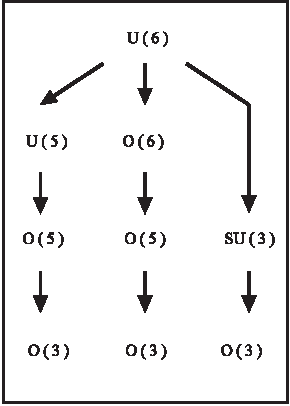
\includegraphics[scale=.65]{figure}
%
% If not, use
%\picplace{5cm}{2cm} % Give the correct figure height and width in cm
%
\caption{If the width of the figure is less than 7.8 cm use the \texttt{sidecapion} command to flush the caption on the left side of the page. If the figure is positioned at the top of the page, align the sidecaption with the top of the figure -- to achieve this you simply need to use the optional argument \texttt{[t]} with the \texttt{sidecaption} command}
\label{fig:1}       % Give a unique label
\end{figure}


\paragraph{Paragraph Heading} %
Instead of simply listing headings of different levels we recommend to let every heading be followed by at least a short passage of text. Furtheron please use the \LaTeX\ automatism for all your cross-references and citations as has already been described in Sect.~\ref{sec:2}.

Please note that the first line of text that follows a heading is not indented, whereas the first lines of all subsequent paragraphs are.

For typesetting numbered lists we recommend to use the \verb|enumerate| environment -- it will automatically render Springer's preferred layout.

\begin{enumerate}
\item{Livelihood and survival mobility are oftentimes coutcomes of uneven socioeconomic development.}
\begin{enumerate}
\item{Livelihood and survival mobility are oftentimes coutcomes of uneven socioeconomic development.}
\item{Livelihood and survival mobility are oftentimes coutcomes of uneven socioeconomic development.}
\end{enumerate}
\item{Livelihood and survival mobility are oftentimes coutcomes of uneven socioeconomic development.}
\end{enumerate}


\subparagraph{Subparagraph Heading} In order to avoid simply listing headings of different levels we recommend to let every heading be followed by at least a short passage of text. Use the \LaTeX\ automatism for all your cross-references and citations as has already been described in Sect.~\ref{sec:2}, see also Fig.~\ref{fig:2}.

Please note that the first line of text that follows a heading is not indented, whereas the first lines of all subsequent paragraphs are.

For unnumbered list we recommend to use the \verb|itemize| environment -- it will automatically render Springer's preferred layout.

\begin{itemize}
\item{Livelihood and survival mobility are oftentimes coutcomes of uneven socioeconomic development, cf. Table~\ref{tab:1}.}
\begin{itemize}
\item{Livelihood and survival mobility are oftentimes coutcomes of uneven socioeconomic development.}
\item{Livelihood and survival mobility are oftentimes coutcomes of uneven socioeconomic development.}
\end{itemize}
\item{Livelihood and survival mobility are oftentimes coutcomes of uneven socioeconomic development.}
\end{itemize}

\begin{figure}[t]
\sidecaption[t]
% Use the relevant command for your figure-insertion program
% to insert the figure file.
% For example, with the option graphics use
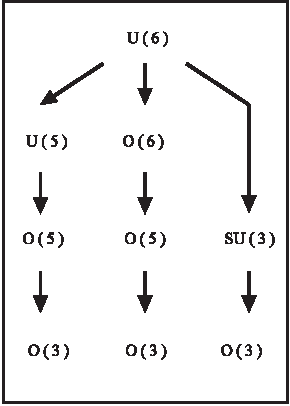
\includegraphics[scale=.65]{figure}
%
% If not, use
%\picplace{5cm}{2cm} % Give the correct figure height and width in cm
%
\caption{Please write your figure caption here}
\label{fig:2}       % Give a unique label
\end{figure}

\runinhead{Run-in Heading Boldface Version} Use the \LaTeX\ automatism for all your cross-references and citations as has already been described in Sect.~\ref{sec:2}.

\subruninhead{Run-in Heading Boldface and Italic Version} Use the \LaTeX\ automatism for all your cross-refer\-ences and citations as has already been described in Sect.~\ref{sec:2}\index{paragraph}.

\subsubruninhead{Run-in Heading Displayed Version} Use the \LaTeX\ automatism for all your cross-refer\-ences and citations as has already been described in Sect.~\ref{sec:2}\index{paragraph}.
% Use the \index{} command to code your index words
%
% For tables use
%
\begin{table}[!t]
\caption{Please write your table caption here}
\label{tab:1}       % Give a unique label
%
% For LaTeX tables use
%
\begin{tabular}{p{2cm}p{2.4cm}p{2cm}p{4.9cm}}
\hline\noalign{\smallskip}
Classes & Subclass & Length & Action Mechanism  \\
\noalign{\smallskip}\svhline\noalign{\smallskip}
Translation & mRNA$^a$  & 22 (19--25) & Translation repression, mRNA cleavage\\
Translation & mRNA cleavage & 21 & mRNA cleavage\\
Translation & mRNA  & 21--22 & mRNA cleavage\\
Translation & mRNA  & 24--26 & Histone and DNA Modification\\
\noalign{\smallskip}\hline\noalign{\smallskip}
\end{tabular}
$^a$ Table foot note (with superscript)
\end{table}
%
\section{Section Heading}
\label{sec:3}
% Always give a unique label
% and use \ref{<label>} for cross-references
% and \cite{<label>} for bibliographic references
% use \sectionmark{}
% to alter or adjust the section heading in the running head
Instead of simply listing headings of different levels we recommend to let every heading be followed by at least a short passage of text. Furtheron please use the \LaTeX\ automatism for all your cross-references and citations as has already been described in Sect.~\ref{sec:2}.

Please note that the first line of text that follows a heading is not indented, whereas the first lines of all subsequent paragraphs are.

If you want to list definitions or the like we recommend to use the Springer-enhanced \verb|description| environment -- it will automatically render Springer's preferred layout.

\begin{description}[Type 1]
\item[Type 1]{That addresses central themes pertainng to migration, health, and disease. In Sect.~\ref{sec:1}, Wilson discusses the role of human migration in infectious disease distributions and patterns.}
\item[Type 2]{That addresses central themes pertainng to migration, health, and disease. In Sect.~\ref{subsec:2}, Wilson discusses the role of human migration in infectious disease distributions and patterns.}
\end{description}

\subsection{Subsection Heading} %
In order to avoid simply listing headings of different levels we recommend to let every heading be followed by at least a short passage of text. Use the \LaTeX\ automatism for all your cross-references and citations citations as has already been described in Sect.~\ref{sec:2}.

Please note that the first line of text that follows a heading is not indented, whereas the first lines of all subsequent paragraphs are.

\begin{svgraybox}
If you want to emphasize complete paragraphs of texts we recommend to use the newly defined Springer class option \verb|graybox| and the newly defined environment \verb|svgraybox|. This will produce a 15 percent screened box 'behind' your text.

If you want to emphasize complete paragraphs of texts we recommend to use the newly defined Springer class option and environment \verb|svgraybox|. This will produce a 15 percent screened box 'behind' your text.
\end{svgraybox}


\subsubsection{Subsubsection Heading}
Instead of simply listing headings of different levels we recommend to let every heading be followed by at least a short passage of text. Furtheron please use the \LaTeX\ automatism for all your cross-references and citations as has already been described in Sect.~\ref{sec:2}.

Please note that the first line of text that follows a heading is not indented, whereas the first lines of all subsequent paragraphs are.

\begin{theorem}
Theorem text goes here.
\end{theorem}
%
% or
%
\begin{definition}
Definition text goes here.
\end{definition}

\begin{proof}
%\smartqed
Proof text goes here.
%\qed
\end{proof}

\paragraph{Paragraph Heading} %
Instead of simply listing headings of different levels we recommend to let every heading be followed by at least a short passage of text. Furtheron please use the \LaTeX\ automatism for all your cross-references and citations as has already been described in Sect.~\ref{sec:2}.

Note that the first line of text that follows a heading is not indented, whereas the first lines of all subsequent paragraphs are.
%
% For built-in environments use
%
\begin{theorem}
Theorem text goes here.
\end{theorem}
%
\begin{definition}
Definition text goes here.
\end{definition}
%
\begin{proof}
%\smartqed
Proof text goes here.
%\qed
\end{proof}
%
%
\begin{trailer}{Trailer Head}
If you want to emphasize complete paragraphs of texts in an \verb|Trailer Head| we recommend to
use  \begin{verbatim}\begin{trailer}{Trailer Head}
...
\end{trailer}\end{verbatim}
\end{trailer}
%
\begin{question}{Questions}
If you want to emphasize complete paragraphs of texts in an \verb|Questions| we recommend to
use  \begin{verbatim}\begin{question}{Questions}
...
\end{question}\end{verbatim}
\end{question}
%
%
\begin{important}{Important}
If you want to emphasize complete paragraphs of texts in an \verb|Important| we recommend to
use  \begin{verbatim}\begin{important}{Important}
...
\end{important}\end{verbatim}
\end{important}
%
\clearpage
\begin{warning}{Attention}
If you want to emphasize complete paragraphs of texts in an \verb|Attention| we recommend to
use  \begin{verbatim}\begin{warning}{Attention}
...
\end{warning}\end{verbatim}
\end{warning}

\begin{programcode}{Program Code}
If you want to emphasize complete paragraphs of texts in an \verb|Program Code| we recommend to
use

\verb|\begin{programcode}{Program Code}|

\verb|\begin{verbatim}...\end{verbatim}|

\verb|\end{programcode}|

\end{programcode}
%
\begin{tips}{Tips}
If you want to emphasize complete paragraphs of texts in an \verb|Tips| we recommend to
use  \begin{verbatim}\begin{tips}{Tips}
...
\end{tips}\end{verbatim}
\end{tips}
%
%
\begin{overview}{Overview}
If you want to emphasize complete paragraphs of texts in an \verb|Overview| we recommend to
use  \begin{verbatim}\begin{overview}{Overview}
...
\end{overview}\end{verbatim}
\end{overview}
\clearpage
\begin{backgroundinformation}{Background Information}
If you want to emphasize complete paragraphs of texts in an \verb|Background|
\verb|Information| we recommend to
use

\verb|\begin{backgroundinformation}{Background Information}|

\verb|...|

\verb|\end{backgroundinformation}|
\end{backgroundinformation}
\begin{legaltext}{Legal Text}
If you want to emphasize complete paragraphs of texts in an \verb|Legal Text| we recommend to
use  \begin{verbatim}\begin{legaltext}{Legal Text}
...
\end{legaltext}\end{verbatim}
\end{legaltext}
%
\begin{acknowledgement}
If you want to include acknowledgments of assistance and the like at the end of an individual chapter please use the \verb|acknowledgement| environment -- it will automatically render Springer's preferred layout.
\end{acknowledgement}
%
\section*{Appendix}
\addcontentsline{toc}{section}{Appendix}
%
When placed at the end of a chapter or contribution (as opposed to at the end of the book), the numbering of tables, figures, and equations in the appendix section continues on from that in the main text. Hence please \textit{do not} use the \verb|appendix| command when writing an appendix at the end of your chapter or contribution. If there is only one the appendix is designated ``Appendix'', or ``Appendix 1'', or ``Appendix 2'', etc. if there is more than one.

\begin{equation}
a \times b = c
\end{equation}
% Problems or Exercises should be sorted chapterwise
\section*{Problems}
\addcontentsline{toc}{section}{Problems}
%
% Use the following environment.
% Don't forget to label each problem;
% the label is needed for the solutions' environment
\begin{prob}
\label{prob1}
A given problem or Excercise is described here. The
problem is described here. The problem is described here.
\end{prob}

\begin{prob}
\label{prob2}
\textbf{Problem Heading}\\
(a) The first part of the problem is described here.\\
(b) The second part of the problem is described here.
\end{prob}

%%%%%%%%%%%%%%%%%%%%%%%% referenc.tex %%%%%%%%%%%%%%%%%%%%%%%%%%%%%%
% sample references
% %
% Use this file as a template for your own input.
%
%%%%%%%%%%%%%%%%%%%%%%%% Springer-Verlag %%%%%%%%%%%%%%%%%%%%%%%%%%
%
% BibTeX users please use
% \bibliographystyle{}
% \bibliography{}
%
\biblstarthook{In view of the parallel print and (chapter-wise) online publication of your book at \url{www.springerlink.com} it has been decided that -- as a genreral rule --  references should be sorted chapter-wise and placed at the end of the individual chapters. However, upon agreement with your contact at Springer you may list your references in a single seperate chapter at the end of your book. Deactivate the class option \texttt{sectrefs} and the \texttt{thebibliography} environment will be put out as a chapter of its own.\\\indent
References may be \textit{cited} in the text either by number (preferred) or by author/year.\footnote{Make sure that all references from the list are cited in the text. Those not cited should be moved to a separate \textit{Further Reading} section or chapter.} If the citatiion in the text is numbered, the reference list should be arranged in ascending order. If the citation in the text is author/year, the reference list should be \textit{sorted} alphabetically and if there are several works by the same author, the following order should be used:
\begin{enumerate}
\item all works by the author alone, ordered chronologically by year of publication
\item all works by the author with a coauthor, ordered alphabetically by coauthor
\item all works by the author with several coauthors, ordered chronologically by year of publication.
\end{enumerate}
The \textit{styling} of references\footnote{Always use the standard abbreviation of a journal's name according to the ISSN \textit{List of Title Word Abbreviations}, see \url{http://www.issn.org/en/node/344}} depends on the subject of your book:
\begin{itemize}
\item The \textit{two} recommended styles for references in books on \textit{mathematical, physical, statistical and computer sciences} are depicted in ~\cite{science-contrib, science-online, science-mono, science-journal, science-DOI} and ~\cite{phys-online, phys-mono, phys-journal, phys-DOI, phys-contrib}.
\item Examples of the most commonly used reference style in books on \textit{Psychology, Social Sciences} are~\cite{psysoc-mono, psysoc-online,psysoc-journal, psysoc-contrib, psysoc-DOI}.
\item Examples for references in books on \textit{Humanities, Linguistics, Philosophy} are~\cite{humlinphil-journal, humlinphil-contrib, humlinphil-mono, humlinphil-online, humlinphil-DOI}.
\item Examples of the basic Springer style used in publications on a wide range of subjects such as \textit{Computer Science, Economics, Engineering, Geosciences, Life Sciences, Medicine, Biomedicine} are ~\cite{basic-contrib, basic-online, basic-journal, basic-DOI, basic-mono}. 
\end{itemize}
}

\begin{thebibliography}{99.}%
% and use \bibitem to create references.
%
% Use the following syntax and markup for your references if 
% the subject of your book is from the field 
% "Mathematics, Physics, Statistics, Computer Science"
%
% Contribution 
\bibitem{science-contrib} Broy, M.: Software engineering --- from auxiliary to key technologies. In: Broy, M., Dener, E. (eds.) Software Pioneers, pp. 10-13. Springer, Heidelberg (2002)
%
% Online Document
\bibitem{science-online} Dod, J.: Effective substances. In: The Dictionary of Substances and Their Effects. Royal Society of Chemistry (1999) Available via DIALOG. \\
\url{http://www.rsc.org/dose/title of subordinate document. Cited 15 Jan 1999}
%
% Monograph
\bibitem{science-mono} Geddes, K.O., Czapor, S.R., Labahn, G.: Algorithms for Computer Algebra. Kluwer, Boston (1992) 
%
% Journal article
\bibitem{science-journal} Hamburger, C.: Quasimonotonicity, regularity and duality for nonlinear systems of partial differential equations. Ann. Mat. Pura. Appl. \textbf{169}, 321--354 (1995)
%
% Journal article by DOI
\bibitem{science-DOI} Slifka, M.K., Whitton, J.L.: Clinical implications of dysregulated cytokine production. J. Mol. Med. (2000) doi: 10.1007/s001090000086 
%
\bigskip

% Use the following (APS) syntax and markup for your references if 
% the subject of your book is from the field 
% "Mathematics, Physics, Statistics, Computer Science"
%
% Online Document
\bibitem{phys-online} J. Dod, in \textit{The Dictionary of Substances and Their Effects}, Royal Society of Chemistry. (Available via DIALOG, 1999), 
\url{http://www.rsc.org/dose/title of subordinate document. Cited 15 Jan 1999}
%
% Monograph
\bibitem{phys-mono} H. Ibach, H. L\"uth, \textit{Solid-State Physics}, 2nd edn. (Springer, New York, 1996), pp. 45-56 
%
% Journal article
\bibitem{phys-journal} S. Preuss, A. Demchuk Jr., M. Stuke, Appl. Phys. A \textbf{61}
%
% Journal article by DOI
\bibitem{phys-DOI} M.K. Slifka, J.L. Whitton, J. Mol. Med., doi: 10.1007/s001090000086
%
% Contribution 
\bibitem{phys-contrib} S.E. Smith, in \textit{Neuromuscular Junction}, ed. by E. Zaimis. Handbook of Experimental Pharmacology, vol 42 (Springer, Heidelberg, 1976), p. 593
%
\bigskip
%
% Use the following syntax and markup for your references if 
% the subject of your book is from the field 
% "Psychology, Social Sciences"
%
%
% Monograph
\bibitem{psysoc-mono} Calfee, R.~C., \& Valencia, R.~R. (1991). \textit{APA guide to preparing manuscripts for journal publication.} Washington, DC: American Psychological Association.
%
% Online Document
\bibitem{psysoc-online} Dod, J. (1999). Effective substances. In: The dictionary of substances and their effects. Royal Society of Chemistry. Available via DIALOG. \\
\url{http://www.rsc.org/dose/Effective substances.} Cited 15 Jan 1999.
%
% Journal article
\bibitem{psysoc-journal} Harris, M., Karper, E., Stacks, G., Hoffman, D., DeNiro, R., Cruz, P., et al. (2001). Writing labs and the Hollywood connection. \textit{J Film} Writing, 44(3), 213--245.
%
% Contribution 
\bibitem{psysoc-contrib} O'Neil, J.~M., \& Egan, J. (1992). Men's and women's gender role journeys: Metaphor for healing, transition, and transformation. In B.~R. Wainrig (Ed.), \textit{Gender issues across the life cycle} (pp. 107--123). New York: Springer.
%
% Journal article by DOI
\bibitem{psysoc-DOI}Kreger, M., Brindis, C.D., Manuel, D.M., Sassoubre, L. (2007). Lessons learned in systems change initiatives: benchmarks and indicators. \textit{American Journal of Community Psychology}, doi: 10.1007/s10464-007-9108-14.
%
%
% Use the following syntax and markup for your references if 
% the subject of your book is from the field 
% "Humanities, Linguistics, Philosophy"
%
\bigskip
%
% Journal article
\bibitem{humlinphil-journal} Alber John, Daniel C. O'Connell, and Sabine Kowal. 2002. Personal perspective in TV interviews. \textit{Pragmatics} 12:257--271
%
% Contribution 
\bibitem{humlinphil-contrib} Cameron, Deborah. 1997. Theoretical debates in feminist linguistics: Questions of sex and gender. In \textit{Gender and discourse}, ed. Ruth Wodak, 99--119. London: Sage Publications.
%
% Monograph
\bibitem{humlinphil-mono} Cameron, Deborah. 1985. \textit{Feminism and linguistic theory.} New York: St. Martin's Press.
%
% Online Document
\bibitem{humlinphil-online} Dod, Jake. 1999. Effective substances. In: The dictionary of substances and their effects. Royal Society of Chemistry. Available via DIALOG. \\
http://www.rsc.org/dose/title of subordinate document. Cited 15 Jan 1999
%
% Journal article by DOI
\bibitem{humlinphil-DOI} Suleiman, Camelia, Daniel C. O'Connell, and Sabine Kowal. 2002. `If you and I, if we, in this later day, lose that sacred fire...': Perspective in political interviews. \textit{Journal of Psycholinguistic Research}. doi: 10.1023/A:1015592129296.
%
%
%
\bigskip
%
%
% Use the following syntax and markup for your references if 
% the subject of your book is from the field 
% "Computer Science, Economics, Engineering, Geosciences, Life Sciences"
%
%
% Contribution 
\bibitem{basic-contrib} Brown B, Aaron M (2001) The politics of nature. In: Smith J (ed) The rise of modern genomics, 3rd edn. Wiley, New York 
%
% Online Document
\bibitem{basic-online} Dod J (1999) Effective Substances. In: The dictionary of substances and their effects. Royal Society of Chemistry. Available via DIALOG. \\
\url{http://www.rsc.org/dose/title of subordinate document. Cited 15 Jan 1999}
%
% Journal article by DOI
\bibitem{basic-DOI} Slifka MK, Whitton JL (2000) Clinical implications of dysregulated cytokine production. J Mol Med, doi: 10.1007/s001090000086
%
% Journal article
\bibitem{basic-journal} Smith J, Jones M Jr, Houghton L et al (1999) Future of health insurance. N Engl J Med 965:325--329
%
% Monograph
\bibitem{basic-mono} South J, Blass B (2001) The future of modern genomics. Blackwell, London 
%
\end{thebibliography}


%%%%%%%%%%%%%%%%%%%%%% appendix.tex %%%%%%%%%%%%%%%%%%%%%%%%%%%%%%%%%
%
% sample appendix
%
% Use this file as a template for your own input.
%
%%%%%%%%%%%%%%%%%%%%%%%% Springer-Verlag %%%%%%%%%%%%%%%%%%%%%%%%%%

\appendix
\motto{All's well that ends well}
\chapter{Chapter Heading}
\label{introA} % Always give a unique label
% use \chaptermark{}
% to alter or adjust the chapter heading in the running head

Use the template \emph{appendix.tex} together with the Springer document class SVMono (monograph-type books) or SVMult (edited books) to style appendix of your book.


\section{Section Heading}
\label{sec:A1}
% Always give a unique label
% and use \ref{<label>} for cross-references
% and \cite{<label>} for bibliographic references
% use \sectionmark{}
% to alter or adjust the section heading in the running head
Instead of simply listing headings of different levels we recommend to let every heading be followed by at least a short passage of text. Furtheron please use the \LaTeX\ automatism for all your cross-references and citations.


\subsection{Subsection Heading}
\label{sec:A2}
Instead of simply listing headings of different levels we recommend to let every heading be followed by at least a short passage of text. Furtheron please use the \LaTeX\ automatism for all your cross-references and citations as has already been described in Sect.~\ref{sec:A1}.

For multiline equations we recommend to use the \verb|eqnarray| environment.
\begin{eqnarray}
\vec{a}\times\vec{b}=\vec{c} \nonumber\\
\vec{a}\times\vec{b}=\vec{c}
\label{eq:A01}
\end{eqnarray}

\subsubsection{Subsubsection Heading}
Instead of simply listing headings of different levels we recommend to let every heading be followed by at least a short passage of text. Furtheron please use the \LaTeX\ automatism for all your cross-references and citations as has already been described in Sect.~\ref{sec:A2}.

Please note that the first line of text that follows a heading is not indented, whereas the first lines of all subsequent paragraphs are.

% For figures use
%
\begin{figure}[t]
\sidecaption[t]
%\centering
% Use the relevant command for your figure-insertion program
% to insert the figure file.
% For example, with the option graphics use
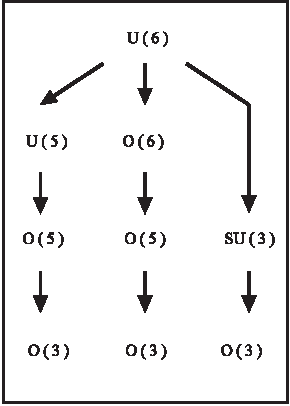
\includegraphics[scale=.65]{figure}
%
% If not, use
%\picplace{5cm}{2cm} % Give the correct figure height and width in cm
%
\caption{Please write your figure caption here}
\label{fig:A1}       % Give a unique label
\end{figure}

% For tables use
%
\begin{table}
\caption{Please write your table caption here}
\label{tab:A1}       % Give a unique label
%
% For LaTeX tables use
%
\begin{tabular}{p{2cm}p{2.4cm}p{2cm}p{4.9cm}}
\hline\noalign{\smallskip}
Classes & Subclass & Length & Action Mechanism  \\
\noalign{\smallskip}\hline\noalign{\smallskip}
Translation & mRNA$^a$  & 22 (19--25) & Translation repression, mRNA cleavage\\
Translation & mRNA cleavage & 21 & mRNA cleavage\\
Translation & mRNA  & 21--22 & mRNA cleavage\\
Translation & mRNA  & 24--26 & Histone and DNA Modification\\
\noalign{\smallskip}\hline\noalign{\smallskip}
\end{tabular}
$^a$ Table foot note (with superscript)
\end{table}
%


\backmatter%%%%%%%%%%%%%%%%%%%%%%%%%%%%%%%%%%%%%%%%%%%%%%%%%%%%%%%
%%%%%%%%%%%%%%%%%%%%%%%acronym.tex%%%%%%%%%%%%%%%%%%%%%%%%%%%%%%%%%%%%%%%%%
% sample list of acronyms
%
% Use this file as a template for your own input.
%
%%%%%%%%%%%%%%%%%%%%%%%% Springer %%%%%%%%%%%%%%%%%%%%%%%%%%

\Extrachap{Glossary}


Use the template \emph{glossary.tex} together with the Springer document class SVMono (monograph-type books) or SVMult (edited books) to style your glossary\index{glossary} in the Springer layout.


\runinhead{glossary term} Write here the description of the glossary term. Write here the description of the glossary term. Write here the description of the glossary term.

\runinhead{glossary term} Write here the description of the glossary term. Write here the description of the glossary term. Write here the description of the glossary term.

\runinhead{glossary term} Write here the description of the glossary term. Write here the description of the glossary term. Write here the description of the glossary term.

\runinhead{glossary term} Write here the description of the glossary term. Write here the description of the glossary term. Write here the description of the glossary term.

\runinhead{glossary term} Write here the description of the glossary term. Write here the description of the glossary term. Write here the description of the glossary term.
%
\Extrachap{Solutions}

\section*{Problems of Chapter~\ref{intro}}

\begin{sol}{prob1}
The solution\index{problems}\index{solutions} is revealed here.
\end{sol}


\begin{sol}{prob2}
\textbf{Problem Heading}\\
(a) The solution of first part is revealed here.\\
(b) The solution of second part is revealed here.
\end{sol}


%\printindex

%%%%%%%%%%%%%%%%%%%%%%%%%%%%%%%%%%%%%%%%%%%%%%%%%%%%%%%%%%%%%%%%%%%%%%



% Disable watermark again at this point
\SetWatermarkText{}

\bibliographystyle{plain}
\bibliography{PrfCmplx-Bakoma}

\end{document}





 
